% !TeX spellcheck = en-US
% !TeX encoding = utf8
% !TeX program = lualatex
% !BIB program = biber
% -*- coding:utf-8 mod:LaTeX -*-


% vv  scroll down to line 200 for content  vv


\let\ifdeutsch\iffalse
\let\ifenglisch\iftrue
% EN: This file is loaded before the \documentclass command in the main document

% EN: The following package allows \\ at the title page
%     For more information see https://github.com/latextemplates/scientific-thesis-cover/issues/4
\RequirePackage{kvoptions-patch}

\ifenglisch
  \PassOptionsToClass{numbers=noenddot}{scrbook}
\else
  %()Aus scrguide.pdf - der Dokumentation von KOMA-Script)
  %Nach DUDEN steht in Gliederungen, in denen ausschließlich arabische Ziffern für die Nummerierung
  %verwendet werden, am Ende der Gliederungsnummern kein abschließender Punkt
  %(siehe [DUD96, R3]). Wird hingegen innerhalb der Gliederung auch mit römischen Zahlen
  %oder Groß- oder Kleinbuchstaben gearbeitet, so steht am Ende aller Gliederungsnummern ein
  %abschließender Punkt (siehe [DUD96, R4])
  \PassOptionsToClass{numbers=autoendperiod}{scrbook}
\fi

% Warns about outdated packages and missing caption declarations
% See https://www.ctan.org/pkg/nag
\RequirePackage[l2tabu, orthodox]{nag}

%DE: Neue deutsche Trennmuster
%    Siehe http://www.ctan.org/pkg/dehyph-exptl und http://projekte.dante.de/Trennmuster/WebHome
%    Nur für pdflatex, nicht für lualatex
\RequirePackage{ifluatex}
\ifluatex
  % do not load anything
\else
  \ifdeutsch
    \RequirePackage[ngerman=ngerman-x-latest]{hyphsubst}
  \fi
\fi

\documentclass[
  % fontsize=11pt is the standard
  a4paper,  % Standard format - only KOMAScript uses paper=a4 - https://tex.stackexchange.com/a/61044/9075
  twoside,  % we are optimizing for both screen and two-side printing. So the page numbers will jump, but the content is configured to stay in the middle (by using the geometry package)
  bibliography=totoc,
  %               idxtotoc,   %Index ins Inhaltsverzeichnis
  %               liststotoc, %List of X ins Inhaltsverzeichnis, mit liststotocnumbered werden die Abbildungsverzeichnisse nummeriert
  headsepline,
  cleardoublepage=empty,
  parskip=half,
  %               draft    % um zu sehen, wo noch nachgebessert werden muss - wichtig, da Bindungskorrektur mit drin
  draft=false
]{scrbook}
% !TeX encoding = utf8
% -*- coding:utf-8 mod:LaTeX -*-

% EN: This file includes basic packages and sets options. The order of package
%     loading is important
% DE: In dieser Datei werden zuerst die benoetigten Pakete eingebunden und
%     danach diverse Optionen gesetzt. Achtung Reihenfolge ist entscheidend!


%%%
% EN: Styleguide:
% - English comments are prefixed with "EN", German comments are prefixed with "DE"
% - Prefixed headings define the language for the subsequent paragraphs
% - It is tried to organize packages in blocks. One block starts with %%%, then
%   % <heading>, then the options and more text. % followed by %%% end a block.
%
% DE: Styleguide:
%
% Ein sehr kleiner Styleguide. Packages werden in Blöcken organisiert.
% Ein Block beginnt mit drei % in einer Zeile, dann % <Blocküberschrift>, dann
% eine Liste der möglichen Optionen und deren Einstellungen, Gründe und Kommentare
% eine % Zeile in der sonst nichts steht und dann wieder %%% in einer Zeile.
%
% Zwischen zwei Blöcken sind 2 Leerzeilen!
% Zu jedem Paket werden soviele Optionen wie möglich/nötig angegeben
%
%%%


%%%
% EN: Enable copy and paste of text from the PDF
%     Only required for pdflatex. It "just works" in the case of lualatex.
%     mmap enables mathematical symbols, but does not work with the newtx font set
%     See: https://tex.stackexchange.com/a/64457/9075
%     Other solutions outlined at http://goemonx.blogspot.de/2012/01/pdflatex-ligaturen-und-copynpaste.html and http://tex.stackexchange.com/questions/4397/make-ligatures-in-linux-libertine-copyable-and-searchable
%     Trouble shooting outlined at https://tex.stackexchange.com/a/100618/9075
\ifluatex
\else
  \usepackage{cmap}
\fi
%%%


%%%
% EN: File encoding
% DE: Codierung
%     Wir sind im 21 Jahrhundert, utf-8 löst so viele Probleme.
%
% Mit UTF-8 funktionieren folgende Pakete nicht mehr. Bitte beachten!
%   * fancyvrb mit §
%   * easylist -> http://www.ctan.org/tex-archive/macros/latex/contrib/easylist/
\ifluatex
  % EN: See https://tex.stackexchange.com/a/158517/9075
  %     Not required, because of usage of fontspec package
  %\usepackage[utf8]{luainputenc}
\else
  \usepackage[utf8]{inputenc}
\fi
%
%%%

%%%
% DE: Parallelbetrieb tex4ht und pdflatex
\makeatletter
\@ifpackageloaded{tex4ht}{
  \def\iftex4ht{\iftrue}
}{
  \def\iftex4ht{\iffalse}
}
\makeatother
%%%


%%%
% EN: Defintion of colors
% DE: Farbdefinitionen
\usepackage[hyperref,dvipsnames]{xcolor}
%

%%%
% EN: Required for custom acronyms/glossaries style.
%     Left aligned Columns in tables with fixed width.
%     See http://tex.stackexchange.com/questions/91566/syntax-similar-to-centering-for-right-and-left
\usepackage{ragged2e}
%%%

%%%
% EN: Abbreviations
% DE: Abkürzungsverzeichnis
%
% DE: Wichtig, ansonsten erscheint "No room for a new \write"
\usepackage{scrwfile}
% DE: siehe http://www.dickimaw-books.com/cgi-bin/faq.cgi?action=view&categorylabel=glossaries#glsnewwriteexceeded
\usepackage[acronym,indexonlyfirst,nomain]{glossaries}
\ifdeutsch
  \renewcommand*{\acronymname}{Abkürzungsverzeichnis}
\else
  \renewcommand*{\acronymname}{List of Abbreviations}
\fi
\renewcommand*{\glsgroupskip}{}
%
% EN: Removed Glossarie as a table as a quick fix to get the template working again
%     See http://tex.stackexchange.com/questions/145579/how-to-print-acronyms-of-glossaries-into-a-table
%
\makenoidxglossaries
%%%


%%%
% EN: Support for language-specific hyphenation
% DE: Neue deutsche Rechtschreibung und Literatur statt "Literature"
%     Die folgende Einstellung ist der Nachfolger von ngerman.sty
\ifdeutsch
  % DE: letzte Sprache ist default, Einbindung von "american" ermöglicht \begin{otherlanguage}{amercian}...\end{otherlanguage} oder \foreignlanguage{american}{Text in American}
  %     Siehe auch http://tex.stackexchange.com/a/50638/9075
  \usepackage[american,ngerman]{babel}
  % Ein "abstract" ist eine "Kurzfassung", keine "Zusammenfassung"
  \addto\captionsngerman{%
    \renewcommand\abstractname{Kurzfassung}%
  }
  \ifluatex
    % EN: conditionally disable ligatures. See https://github.com/latextemplates/scientific-thesis-template/issues/54
    %     for a discussion
    \usepackage[ngerman]{selnolig}
  \fi
\else
  % EN: Set English as language and allow to write hyphenated"=words
  %     `american`, `english` and `USenglish` are synonyms for babel package (according to https://tex.stackexchange.com/questions/12775/babel-english-american-usenglish).
  %      "english" has to go last to set it as default language
  \usepackage[ngerman,english]{babel}
  % EN: Hint by http://tex.stackexchange.com/a/321066/9075 -> enable "= as dashes
  \addto\extrasenglish{\languageshorthands{ngerman}\useshorthands{"}}
  \ifluatex
    % EN: conditionally disable ligatures. See https://github.com/latextemplates/scientific-thesis-template/issues/54
    %     for a discussion
    \usepackage[english]{selnolig}
  \fi
\fi
%
%%%


%%%
% EN: For easy quotations: \enquote{text}
%     This package is very smart when nesting is applied, otherwise textcmds (see below) provides a shorter command
% DE:  Anführungszeichen
%      Zitate in \enquote{...} setzen, dann werden automatisch die richtigen Anführungszeichen verwendet.
\usepackage{csquotes}
%%%


%%%
% EN: For even easier quotations: \qq{text}.
%     Is not smart in the case of nesting, but good enough for the most cases
\usepackage{textcmds}
\ifdeutsch
  % EN: German quotes are different. So do not use the English quotes, but the ones provided by the csquotes package.
  \renewcommand{\qq}[1]{\enquote{#1}}
\fi
%%%


%%%
% EN: extended enumarations
% DE: erweitertes Enumerate
\usepackage{paralist}
%
%%%


%%%
% DE: fancyheadings (nicht nur) fuer koma
\usepackage[automark]{scrlayer-scrpage}
%
%%%


%%%
% EN: Mathematics
% DE: Mathematik
%
% DE: Viele Mathematik-Sachen. Siehe https://texdoc.net/pkg/amsmath
\usepackage{amsmath}
% EN: Options must be passed this way, otherwise it does not work with glossaries
\PassOptionsToPackage{fleqn,leqno}{amsmath}
% DE: fleqn (=Gleichungen linksbündig platzieren) funktioniert nicht direkt. Es muss noch ein Patch gemacht werden:
%\addtolength\mathindent{1em}%work-around ams-math problem with align and 9 -> 10. Does not work with glossaries, No visual changes.
% EN: Fixes bugs in AMS math
\usepackage{mathtools}
%
% EN: For theorems, replacement for amsthm
\usepackage[amsmath,hyperref]{ntheorem}
\theorempreskipamount 2ex plus1ex minus0.5ex
\theorempostskipamount 2ex plus1ex minus0.5ex
\theoremstyle{break}
\newtheorem{definition}{Definition}[section]
%
%%%


%%%
% DE: Intelligentes Leerzeichen um hinter Abkürzungen die richtigen Abstände zu erhalten, auch leere.
%     Siehe commands.tex \gq{}
\usepackage{xspace}
%DE: Macht \xspace und \enquote kompatibel
\makeatletter
\xspaceaddexceptions{\grqq \grq \csq@qclose@i \} }
\makeatother
%
%%%


%%%
% EN: Package for the appendix
% DE: Anhang
\usepackage{appendix}
%[toc,page,title,header]
%
%%%

%%%
% EN: Graphics
% DE: Grafikeinbindungen
%
% EN: The parameter "pdftex" is not required
\usepackage{graphicx}
\graphicspath{{\getgraphicspath}}
\newcommand{\getgraphicspath}{graphics/}
%
%%%


%%%
% EN: Enables inclusion of SVG graphics - 1:1 approach
%    This is NOT the approach of https://ctan.org/pkg/svg-inkscape,
%     which allows text in SVG to be typeset using LaTeX
%     We just include the SVG as is.
\usepackage{epstopdf}
\epstopdfDeclareGraphicsRule{.svg}{pdf}{.pdf}{%
  inkscape -z -D --file=#1 --export-pdf=\OutputFile
}
%
%%%


%%%
% EN: Enables inclusion of SVG graphics - text-rendered-with-LaTeX-approach
%     This is the approach of https://ctan.org/pkg/svg-inkscape,
\newcommand{\executeiffilenewer}[3]{%
  \IfFileExists{#2}
  {
    %\message{file #2 exists}
    \ifnum\pdfstrcmp{\pdffilemoddate{#1}}%
      {\pdffilemoddate{#2}}>0%
      {\immediate\write18{#3}}
    \else
      {%\message{file up to date #2}
      }
    \fi%
  }{
    %\message{file #2 doesn't exist}
    %\message{argument: #3}
    %\immediate\write18{echo "test" > xoutput.txt}
    \immediate\write18{#3}
  }
}
\newcommand{\includesvg}[1]{%
  \executeiffilenewer{#1.svg}{#1.pdf}%
  {
    inkscape -z -D --file=\getgraphicspath#1.svg %
    --export-pdf=\getgraphicspath#1.pdf --export-latex}%
  \input{\getgraphicspath#1.pdf_tex}%
}


%%%
% EN: Enable typesetting values with SI units.
\ifdeutsch
  \usepackage[mode=text,group-four-digits]{siunitx}
  \sisetup{locale=DE}
\else
  \usepackage[mode=text,group-four-digits,group-separator={,}]{siunitx}
  \sisetup{locale=US}
\fi
%%%

%%%
% EN: Extensions for tables
% DE: Tabellenerweiterungen
\usepackage{array} %increases tex's buffer size and enables ``>'' in tablespecs
\usepackage{longtable}
\usepackage{dcolumn} %Aligning numbers by decimal points in table columns
\ifdeutsch
  \newcolumntype{d}[1]{D{.}{,}{#1}}
\else
  \newcolumntype{d}[1]{D{.}{.}{#1}}
\fi
\setlength{\extrarowheight}{1pt}
%%%

%%%
% Eine Zelle, die sich über mehrere Zeilen erstreckt.
% Siehe Beispieltabelle in Kapitel 2
\usepackage{multirow}
%
%%%

%%%
%Fuer Tabellen mit Variablen Spaltenbreiten
%\usepackage{tabularx}
%\usepackage{tabulary}
%
%%%


%%%
% EN: Links behave as they should. Enables "\url{...}" for URL typesettings.
%     Allow URL breaks also at a hyphen, even though it might be confusing: Is the "-" part of the address or just a hyphen?
%     See https://tex.stackexchange.com/a/3034/9075.
% DE: Links verhalten sich so, wie sie sollen
%     Zeilenumbrüche bei URLs auch bei Bindestrichen erlauben, auch wenn es verwirrend sein könnte: Gehört der Bindestrich zur URL oder ist es ein Trennstrich?
%     Siehe https://tex.stackexchange.com/a/3034/9075.
\usepackage[hyphens]{url}
%
%  EN: When activated, use text font as url font, not the monospaced one.
%      For all options see https://tex.stackexchange.com/a/261435/9075.
% \urlstyle{same}
%
% EN: Hint by http://tex.stackexchange.com/a/10419/9075.
\makeatletter
\g@addto@macro{\UrlBreaks}{\UrlOrds}
\makeatother
%
%%%


%%%
% Index über Begriffe, Abkürzungen
%\usepackage{makeidx} makeidx ist out -> http://xindy.sf.net verwenden
%
%%%

%%%
%lustiger Hack fuer das Abkuerzungsverzeichnis
%nach latex durchlauf folgendes ausfuehren
%makeindex ausarbeitung.nlo -s nomencl.ist -o ausarbeitung.nls
%danach nochmal latex
%\usepackage{nomencl}
%    \let\abk\nomenclature %Deutsche Ueberschrift setzen
%          \renewcommand{\nomname}{List of Abbreviations}
%        %Punkte zw. Abkuerzung und Erklaerung
%          \setlength{\nomlabelwidth}{.2\hsize}
%          \renewcommand{\nomlabel}[1]{#1 \dotfill}
%        %Zeilenabstaende verkleinern
%          \setlength{\nomitemsep}{-\parsep}
%    \makenomenclature
%
%%%

%%%
% EN: Logic for TeX - enables if-then-else in commands
% DE: Logik für TeX
%     FÜr if-then-else @ commands.tex
\usepackage{ifthen}
%
%%%


%%%
% EN: Code Listings
% DE: Listings
\usepackage{listings}
\lstset{language=XML,
  showstringspaces=false,
  extendedchars=true,
  basicstyle=\footnotesize\ttfamily,
  commentstyle=\slshape,
  % DE: Original: \rmfamily, damit werden die Strings im Quellcode hervorgehoben. Zusaetzlich evtl.: \scshape oder \rmfamily durch \ttfamily ersetzen. Dann sieht's aus, wie bei fancyvrb
  stringstyle=\ttfamily,
  breaklines=true,
  breakatwhitespace=true,
  % EN: alternative: fixed
  columns=flexible,
  numbers=left,
  numberstyle=\tiny,
  basewidth=.5em,
  xleftmargin=.5cm,
  % aboveskip=0mm, %DE: deaktivieren, falls man lstlistings direkt als floating object benutzt (\begin{lstlisting}[float,...])
  % belowskip=0mm, %DE: deaktivieren, falls man lstlistings direkt als floating object benutzt (\begin{lstlisting}[float,...])
  captionpos=b
}

\ifluatex
\else
  % EN: Enable UTF-8 support - see https://tex.stackexchange.com/q/419327/9075
  \usepackage{listingsutf8}
  \lstset{inputencoding=utf8/latin1}
\fi

\ifdeutsch
  \renewcommand{\lstlistlistingname}{Verzeichnis der Listings}
\fi
%
%%%


%%%
% EN: Alternative to listings could be fancyvrb. Can be used together.
% DE: Alternative zu Listings ist fancyvrb. Kann auch beides gleichzeitig benutzt werden.
\usepackage{fancyvrb}
%
%EN: Font size for the normal text
%DE: Groesse fuer den Fliesstext. Falls deaktiviert: \normalsize
%\fvset{fontsize=\small}
%
%DE: Somit kann im Text ganz einfach §verbatim§ text gesetzt werden.
%    Disabled, because UTF-8 does not work any more and lualatex causes issues
%\DefineShortVerb{\§}
%
%EN: Shrink font size of listings
\RecustomVerbatimEnvironment{Verbatim}{Verbatim}{fontsize=\footnotesize}
\RecustomVerbatimCommand{\VerbatimInput}{VerbatimInput}{fontsize=\footnotesize}
%
%EN: Hack for fancyvrb based on http://newsgroups.derkeiler.com/Archive/Comp/comp.text.tex/2008-12/msg00075.html
%EN: Change of the solution: \Vref somehow collidated with cleveref/varioref as the output of \Vref{} was "Abschnitt 4.3 auf Seite 85"; therefore changed to \myVref -- so completely removed
\newcommand{\Vlabel}[1]{\label[line]{#1}\hypertarget{#1}{}}
\newcommand{\lref}[1]{\hyperlink{#1}{\FancyVerbLineautorefname~\ref*{#1}}}
%
%%%


%%%
% EN: Tunings of captions for floats, listings, ...
% DE: Bildunterschriften bei floats genauso formatieren wie bei Listings
%     Anpassung wird unten bei den newfloat-Deklarationen vorgenommen
%     https://www.ctan.org/pkg/caption2 is superseeded by this package.
\usepackage{caption}
%
%%%


%%%
% EN: Provides rotating figures, where the PDF page is also turned
% DE: Ermoeglicht es, Abbildungen um 90 Grad zu drehen
%     Alternatives Paket: rotating Allerdings wird hier nur das Bild gedreht, während bei lscape auch die PDF-Seite gedreht wird.
%     Das Paket lscape dreht die Seite auch nicht
\usepackage{pdflscape}
%
%%%


%%%
%EN: Required for proper environments of fancyvrb and lstlistings
%    There is also the newfloat pacakge (recommended by minted), but we currently have no expericene with that
%DE: Wird für fancyvrb und für lstlistings verwendet
\usepackage{float}
%
% EN: Alternative to float package
%\usepackage{floatrow}
%DE: zustäzlich für den Paramter [H] = Floats WIRKLICH da wo sie deklariert wurden paltzieren - ganz ohne Kompromisse
%    floatrow ist der Nachfolger von float
%    Allerdings macht floatrow in manchen Konstellationen Probleme. Deshalb ist das Paket deaktiviert.
%
% EN: See http://www.tex.ac.uk/cgi-bin/texfaq2html?label=floats
% DE: floats IMMER nach einer Referenzierung platzieren
%\usepackage{flafter}
%%%


%%%
% EN: For nested figures
% DE: Fuer Abbildungen innerhalb von Abbildungen
%     Ersetzt die Pakete subfigure und subfig - siehe https://tex.stackexchange.com/a/13778/9075
\usepackage[hypcap=true]{subcaption}
%
%%%


%%%
% EN: Extended support for footnotes
% DE: Fußnoten
%
%\usepackage{dblfnote}  %Zweispaltige Fußnoten
%
% Keine hochgestellten Ziffern in der Fußnote (KOMA-Script-spezifisch):
%\deffootnote[1.5em]{0pt}{1em}{\makebox[1.5em][l]{\bfseries\thefootnotemark}}
%
% Abstand zwischen Fußnoten vergrößern:
%\setlength{\footnotesep}{.85\baselineskip}
%
% EN: Following command disables the separting line of the footnote
% DE: Folgendes Kommando deaktiviert die Trennlinie zur Fußnote
%\renewcommand{\footnoterule}{}
%
\addtolength{\skip\footins}{\baselineskip} % Abstand Text <-> Fußnote
%
% Fußnoten immer ganz unten auf einer \raggedbottom-Seite
% fnpos kommt aus dem yafoot package
\usepackage{fnpos}
\makeFNbelow
\makeFNbottom
%
%%%


%%%
% EN: Variable page heights
% DE: Variable Seitenhöhen zulassen
\raggedbottom
%
%%%


%%%
% Falls die Seitenzahl bei einer Referenz auf eine Abbildung nur dann angegeben werden soll,
% falls sich die Abbildung nicht auf der selben Seite befindet...
\iftex4ht
  %tex4ht does not work well with vref, therefore we emulate vref behavior
  \newcommand{\vref}[1]{\ref{#1}}
\else
  \ifdeutsch
    \usepackage[ngerman]{varioref}
  \else
    \usepackage{varioref}
  \fi
\fi
%%%

%%%
% EN: More beautiful tables if one uses \toprule, \midrule, \bottomrule
% DE: Noch schoenere Tabellen als mit booktabs mit http://www.zvisionwelt.de/downloads.html
\usepackage{booktabs}
%
%\usepackage[section]{placeins}
%
%%%


%%%
% EN: Graphs and Automata
%
% TODO: Since version 3.0 (2013-10-01), it supports pdflatex via the auto-pst-pdf package
%       Requires -shell-escape
%\usepackage{gastex}
%%%


%%%
%
%\usepackage{multicol}
%\usepackage{setspace} % kollidiert mit diplomarbeit.sty
%%%


%%%
%biblatex statt bibtex
\usepackage[
  backend       = biber, %biber does not work with 64x versions alternative: bibtex8
  %minalphanames only works with biber backend
  sortcites     = true,
  bibstyle      = alphabetic,
  citestyle     = alphabetic,
  giveninits    = true,
  useprefix     = false, %"von, van, etc." will be printed, too. See below.
  minnames      = 1,
  minalphanames = 3,
  maxalphanames = 4,
  maxbibnames   = 99,
  maxcitenames  = 2,
  natbib        = true,
  eprint        = true,
  url           = true,
  doi           = true,
  isbn          = true,
  backref       = true]{biblatex}

% enable more breaks at URLs. See https://tex.stackexchange.com/a/134281.
\setcounter{biburllcpenalty}{7000}
\setcounter{biburlucpenalty}{8000}

\bibliography{bibliography}
%\addbibresource[datatype=bibtex]{bibliography.bib}

%Do not put "vd" in the label, but put it at "\citeauthor"
%Source: http://tex.stackexchange.com/a/30277/9075
\makeatletter
\AtBeginDocument{\toggletrue{blx@useprefix}}
\AtBeginBibliography{\togglefalse{blx@useprefix}}
\makeatother

%Thin spaces between initials
%http://tex.stackexchange.com/a/11083/9075
\renewrobustcmd*{\bibinitdelim}{\,}

%Keep first and last name together in the bibliography
%http://tex.stackexchange.com/a/196192/9075
\renewcommand*\bibnamedelimc{\addnbspace}
\renewcommand*\bibnamedelimd{\addnbspace}

%Replace last "and" by comma in bibliography
%See http://tex.stackexchange.com/a/41532/9075
\AtBeginBibliography{%
  \renewcommand*{\finalnamedelim}{\addcomma\space}%
}

\DefineBibliographyStrings{ngerman}{
  backrefpage  = {zitiert auf S\adddot},
  backrefpages = {zitiert auf S\adddot},
  andothers    = {et\ \addabbrvspace al\adddot},
  %Tipp von http://www.mrunix.de/forums/showthread.php?64665-biblatex-Kann-%DCberschrift-vom-Inhaltsverzeichnis-nicht-%E4ndern&p=293656&viewfull=1#post293656
  bibliography = {Literaturverzeichnis}
}

%enable hyperlinked author names when using \citeauthor
%source: http://tex.stackexchange.com/a/75916/9075
\DeclareCiteCommand{\citeauthor}
{\boolfalse{citetracker}%
  \boolfalse{pagetracker}%
  \usebibmacro{prenote}}
{\ifciteindex
  {\indexnames{labelname}}
  {}%
  \printtext[bibhyperref]{\printnames{labelname}}}
{\multicitedelim}
{\usebibmacro{postnote}}

%natbib compatibility
%\newcommand{\citep}[1]{\cite{#1}}
%\newcommand{\citet}[1]{\citeauthor{#1} \cite{#1}}
%Beginning of sentence - analogous to cleveref - important for names such as "zur Muehlen"
%\newcommand{\Citep}[1]{\cite{#1}}
%\newcommand{\Citet}[1]{\Citeauthor{#1} \cite{#1}}
%%%


%%%
% DE: Blindtext. Paket "blindtext" ist fortgeschritterner als "lipsum" und kann auch Mathematik im Text (http://texblog.org/2011/02/26/generating-dummy-textblindtext-with-latex-for-testing/)
%     kantlipsum (https://www.ctan.org/tex-archive/macros/latex/contrib/kantlipsum) ist auch ganz nett, aber eben auch keine Mathematik
%     Wird verwendet, um etwas Text zu erzeugen, um eine volle Seite wegen Layout zu sehen.
\usepackage[math]{blindtext}
%%%


%%%
% EN: Make LaTeX logos available by commands. E.g., \lualatex
\usepackage{dtk-logos}
%
%%%


%%%
% DE: Neue Pakete bitte VOR hyperref einbinden. Insbesondere bei Verwendung des
%     Pakets "index" wichtig, da sonst die Referenzierung nicht funktioniert.
%     Für die Indizierung selbst ist unter http://xindy.sourceforge.net
%     ein gutes Tool zu erhalten
%%%


%%%
%
% EN: Add new packages at this place
% DE: Hier also neue packages einbinden
%
%%%


%%%
% EN: Provides hyperlinks
%     Option "unicode" fixes umlauts in the PDF bookmarks - see https://tex.stackexchange.com/a/338770/9075
%
% DE: Erlaubt Hyperlinks im Dokument.
%     Alle Optionen nach \hypersetup verschoben, sonst crash
%     Siehe auch: "Praktisches LaTeX" - www.itp.uni-hannover.de/~kreutzm
\usepackage[unicode]{hyperref}
%

% EN: Define colors
% DE: Da es mit KOMA 3 und xcolor zu Problemen mit den global Options kommt MÜSSEN die Optionen so gesetzt werden.
%     Eigene Farbdefinitionen ohne die Namen des xcolor packages
\definecolor{darkblue}{rgb}{0,0,.5}
\definecolor{black}{rgb}{0,0,0}

% EN: Define color of links and more
\hypersetup{
  bookmarksnumbered=true,
  bookmarksopen=true,
  bookmarksopenlevel=1,
  breaklinks=true,
  colorlinks=true,
  pdfstartview=Fit,
  pdfpagelayout=SinglePage, % DE: Alterntaive: TwoPageRight -- zweiseitige Darstellung: ungerade Seiten rechts im PDF-Viewer - siehe auch http://tex.stackexchange.com/a/21109/9075
  %pdfencoding=utf8, % EN: This is probably the same as passing the option "unicode" at \usepackage{hyperref}
  filecolor=darkblue,
  urlcolor=darkblue,
  linkcolor=black,
  citecolor=black
}
%
%%%

%%%
% EN: Extensions for references inside the document (\cref{fig:sample}, ...)
% DE: cleveref für cref statt autoref, da cleveref auch bei Definitionen funktioniert
\ifdeutsch
  \usepackage[ngerman,capitalise,nameinlink,noabbrev]{cleveref}
\else
  \usepackage[capitalise,nameinlink,noabbrev]{cleveref}
\fi
%%%


%%%
% DE: Zur Darstellung von Algorithmen
%     Algorithm muss nach hyperref geladen werden
\usepackage[chapter]{algorithm}
\usepackage[]{algpseudocode}
%
%%%


%%%%%%%%%%%%%%%%%%%%%%%%%%%%%%%%%%%%%%%%%%%%%%%%%%%%%%%%%%%%%%%%%%%%%%%%%%%%%
%% EN: Fonts
%% DE: Schriften
%%
%% !!! If you change the font, be sure that words such as "workflow" can
%% !!! still be copied from the PDF. If this is not the case, you have
%% !!! to use glyphtounicode. See comment at cmap package
%%%%%%%%%%%%%%%%%%%%%%%%%%%%%%%%%%%%%%%%%%%%%%%%%%%%%%%%%%%%%%%%%%%%%%%%%%%%%

\automark[section]{chapter}
\setkomafont{pageheadfoot}{\normalfont\sffamily}
\setkomafont{pagenumber}{\normalfont\sffamily}
%
%\setheadsepline[.4pt]{.4pt} %funktioniert nicht: Alle Linien sind hier weg
%
%%%

%%%
% DE: Fuer deutsche Texte: Weniger Silbentrennung, mehr Abstand zwischen den Woertern
\ifdeutsch
  \setlength{\emergencystretch}{3em} % Silbentrennung reduzieren durch mehr frei Raum zwischen den Worten
\fi
%%%

% EN: Times Roman for all text
\ifluatex
  \usepackage{fontspec}
  \setmainfont{TeX Gyre Termes}
  \setsansfont[Scale=.9]{TeX Gyre Heros}
  \setmonofont[StylisticSet={1,3},Scale=.9]{inconsolata}
  \RequirePackage{newtxmath}
\else
  \RequirePackage{newtxtext}
  \RequirePackage{newtxmath}
  % EN: looks good with times, but no equivalent for lualatex found,
  %     therefore replaced with inconsolata
  %\RequirePackage[zerostyle=b,scaled=.9]{newtxtt}
  \RequirePackage[varl,scaled=.9]{inconsolata}
\fi

% EN: Fallback font - if the subsequent font packages do not define a font (e.g., monospaced)
%     This is the modern package for "Computer Modern".
% DE: Fallback-Schriftart
%\usepackage[%
%    rm={oldstyle=false,proportional=true},%
%    sf={oldstyle=false,proportional=true},%
%    tt={oldstyle=false,proportional=true,variable=true},%
%    qt=false%
%]{cfr-lm}

% EN: Headings are typset in Helvetica (which is similar to Arial)
% DE: Schriftart fuer die Ueberschriften - ueberschreibt lmodern
%\usepackage[scaled=.95]{helvet}

% DE: Für Schreibschrift würde tun, muss aber nicht
%\usepackage{mathrsfs} %  \mathscr{ABC}

% EN: Font for the main text
% DE: Schriftart fuer den Fliesstext - ueberschreibt lmodern
%     Linux Libertine, siehe http://www.linuxlibertine.org/
%     Packageparamter [osf] = Minuskel-Ziffern
%     rm = libertine im Brottext, Linux Biolinum NICHT als serifenlose Schrift, sondern helvet (von oben) beibehalten
%\usepackage[rm]{libertine}

% EN: Alternative Font: Palantino. It is recommeded by Prof. Ludewig for German texts
% DE: Alternative Schriftart: Palantino, Packageparamter [osf] = Minuskel-Ziffern
%     Bitte nur in deutschen Texten
%\usepackage{mathpazo} %ftp://ftp.dante.de/tex-archive/fonts/mathpazo/ - Tipp aus DE-TEX-FAQ 8.2.1

% DE: Schriftart fuer Programmcode - ueberschreibt lmodern
%     Falls auskommentiert, wird die Standardschriftart lmodern genommen
%     Fuer schreibmaschinenartige Schluesselwoerter in den Listings - geht bei alten Installationen nicht, da einige Fontshapes (<>=) fehlen
%\usepackage[scaled=.92]{luximono}
%\usepackage{courier}
% DE: BeraMono als Typewriter-Schrift, Tipp von http://tex.stackexchange.com/a/71346/9075
%\usepackage[scaled=0.83]{beramono}

% EN: backticks (`) are rendered as such in verbatim environments.
%     See following links for details:
%     - https://tex.stackexchange.com/a/341057/9075
%     - https://tex.stackexchange.com/a/47451/9075
%     - https://tex.stackexchange.com/a/166791/9075
\usepackage{upquote}

% DE: Symbole
%
%\usepackage[geometry]{ifsym} % \BigSquare
%\usepackage{mathabx}
%\usepackage{stmaryrd} %fuer \ovee, \owedge, \otimes
%\usepackage{marvosym} %fuer \Writinghand %patched to not redefine \Rightarrow
%\usepackage{mathrsfs} %mittels \mathscr{} schoenen geschwungenen Buchstaben erzeugen
%\usepackage{calrsfs} %\mathcal{} ein bisserl dickeren buchstaben erzeugen - sieht net so gut aus.
%durch mathpazo ist das schon definiert
\usepackage{amssymb}

% EN: For \texttrademark{}
\usepackage{textcomp}

% EN: name-clashes von marvosym und mathabx vermeiden:
\def\delsym#1{%
  %  \expandafter\let\expandafter\origsym\expandafter=\csname#1\endcsname
  %  \expandafter\let\csname orig#1\endcsname=\origsym
  \expandafter\let\csname#1\endcsname=\relax
}

%\usepackage{pifont}
%\usepackage{bbding}
%\delsym{Asterisk}
%\delsym{Sun}\delsym{Mercury}\delsym{Venus}\delsym{Earth}\delsym{Mars}
%\delsym{Jupiter}\delsym{Saturn}\delsym{Uranus}\delsym{Neptune}
%\delsym{Pluto}\delsym{Aries}\delsym{Taurus}\delsym{Gemini}
%\delsym{Rightarrow}
%\usepackage{mathabx} - Ueberschreibt leider zu viel - und die \le-Zeichen usw. sehen nicht gut aus!


%%%
% EN: Modern font encoding
%     Has to be loaded AFTER any font packages. See https://tex.stackexchange.com/a/2869/9075.
\ifluatex
\else
  \usepackage[T1]{fontenc}
\fi
%
%%%

%%
% EN: Character protrusion and font expansion. See http://www.ctan.org/tex-archive/macros/latex/contrib/microtype/
\usepackage[
  babel=true, % EN: Enable language-specific kerning. Take language-settings from the languge of the current document (see Section 6 of microtype.pdf)
  expansion=alltext,
  protrusion=alltext-nott, % EN: Ensure that at listings, there is no change at the margin of the listing
  final % EN: Always enable microtype, even if in draft mode. This helps finding bad boxes quickly.
        %     In the standard configuration, this template is always in the final mode, so this option only makes a difference if "pros" use the draft mode
]{microtype}
%
% EN: \texttt{test -- test} keeps the "--" as "--" (and does not convert it to an en dash)
\DisableLigatures{encoding = T1, family = tt* }
%
%DE: fuer microtype
%DE: tracking=true muss als Parameter des microtype-packages mitgegeben werden
%DE: Deaktiviert, da dies bei Algorithmen seltsam aussieht
%
%\DeclareMicrotypeSet*[tracking]{my}{ font = */*/*/sc/* }%
%\SetTracking{ encoding = *, shape = sc }{ 45 }
%DE: Hier wird festgelegt,
%    dass alle Passagen in Kapitälchen automatisch leicht
%    gesperrt werden.
%    Quelle: http://homepage.ruhr-uni-bochum.de/Georg.Verweyen/pakete.html
%    Deaktiviert, da sonst "BPEL", "BPMN" usw. wirklich komisch aussehen.
%    Macht wohl nur bei geisteswissenschaftlichen Arbeiten Sinn.
%%%

%%%
% CTAN: https://ctan.org/pkg/lccaps
% Doc: http://texdoc.net/pkg/lccaps
%
% Required for DE/EN \initialism
\usepackage{lccaps}
%%%

%%%
% Links auf Gleitumgebungen springen nicht zur Beschriftung,
% Doc: http://mirror.ctan.org/tex-archive/macros/latex/contrib/oberdiek/hypcap.pdf
% sondern zum Anfang der Gleitumgebung
\usepackage[all]{hypcap}
%%%


%%%
% Deckblattstyle
%
\ifdeutsch
  \PassOptionsToPackage{language=german}{scientific-thesis-cover}
\else
  \PassOptionsToPackage{language=english}{scientific-thesis-cover}
\fi


%%%
%Bugfixes packages
%\usepackage{fixltx2e} %Fuer neueste LaTeX-Installationen nicht mehr benoetigt - bereinigte einige Ungereimtheiten, die auf Grund von Rueckwaertskompatibilitaet beibahlten wurden.
%\usepackage{mparhack} %Fixt die Position von marginpars (die in DAs selten bis gar nicht gebraucht werden}
%\usepackage{ellipsis} %Fixt die Abstaende vor \ldots. Wird wohl auch nicht benoetigt.
%
%%%


%%%
% EN: Settings for captions of floats
% DE: Formatierung der Beschriftungen
%
\captionsetup{
  format=hang,
  labelfont=bf,
  justification=justified,
  %single line captions should be centered, multiline captions justified
  singlelinecheck=true
}
%
% EN: New float environments for listings and algorithms
%
% \floatstyle{ruled} % TODO: enabled or disabled causes no change - listings and algorithms are always ruled
%
\newfloat{Listing}{tbp}{code}[chapter]
\crefname{Listing}{Listing}{Listings}
%
\newfloat{Algorithmus}{tbp}{alg}[chapter]
\ifdeutsch
  \crefname{Algorithmus}{Algorithmus}{Algorithmus}
\else
  \crefname{Algorithmus}{Algorithm}{Algorithms}
  \floatname{Algorithmus}{Algorithm}
\fi
%%


%%
%amsmath
%\numberwithin{equation}{section}
%\renewcommand{\theequation}{\thesection.\Roman{equation}}
%%


%%%
%EN: Various chapter styles
% DE: unterschiedliche Chapter-Styles
%     u.a. Paket fncychap

% Andere Kapitelueberschriften
% falls einem der Standard von KOMA nicht gefaellt...
% Falls man zurück zu KOMA moechte, dann muss jede der vier folgenden Moeglichkeiten deaktiviert sein.

%\usepackage[Sonny]{fncychap}

%\usepackage[Bjarne]{fncychap}

%\usepackage[Lenny]{fncychap}

%DE: Zur Aktivierung eines der folgenden Möglichkeiten ein Paar von "\iffalse" und "\fi" auskommentieren

\iffalse
  \usepackage[Bjarne]{fncychap}
  \ChNameVar{\Large\sf} \ChNumVar{\Huge} \ChTitleVar{\Large\sf}
  \ChRuleWidth{0.5pt} \ChNameUpperCase
\fi

\iffalse
  \usepackage[Rejne]{fncychap}
  \ChNameVar{\centering\Huge\rm\bfseries}
  \ChNumVar{\Huge}
  \ChTitleVar{\centering\Huge\rm}
  \ChNameUpperCase
  \ChTitleUpperCase
  \ChRuleWidth{1pt}
\fi

\iffalse
  \usepackage{fncychap}
  \ChNameUpperCase
  \ChTitleUpperCase
  \ChNameVar{\raggedright\normalsize} %\rm
  \ChNumVar{\bfseries\Large}
  \ChTitleVar{\raggedright\Huge}
  \ChRuleWidth{1pt}
\fi

\iffalse
  \usepackage[Bjornstrup]{fncychap}
  \ChNumVar{\fontsize{76}{80}\selectfont\sffamily\bfseries}
  \ChTitleVar{\raggedright\Large\sffamily\bfseries}
\fi

% EN: Complete different chapter style - self made

% Innen drin kann man dann noch zwischen
%   * serifenloser Schriftart (eingestellt)
%   * serifenhafter Schriftart (wenn kein zusaetzliches Kommando aktiviert ist) und
%   * Kapitälchen wählen
\iffalse
  \makeatletter
  %\def\thickhrulefill{\leavevmode \leaders \hrule height 1ex \hfill \kern \z@}

  %Fuer Kapitel mit Kapitelnummer
  \def\@makechapterhead#1{%
    \vspace*{10\p@}%
    {\parindent \z@ \raggedright \reset@font
      %Default-Schrift: Serifenhaft (gut fuer englische Dokumente)
      %A) Fuer serifenlose Schrift:
      \fontfamily{phv}\selectfont
      %B) Fuer Kapitaelchen:
      %\fontseries{m}\fontshape{sc}\selectfont
      %C) Fuer ganz "normale" Schrift:
      %\normalfont
      %
      \Large \@chapapp{} \thechapter
      \par\nobreak\vspace*{10\p@}%
      \interlinepenalty\@M
      {\Huge\bfseries\baselineskip3ex
        %Fuer Kapitaelchen folgende Zeile aktivieren:
        %\fontseries{m}\fontshape{sc}\selectfont
        #1\par\nobreak}
      \vspace*{10\p@}%
      \makebox[\textwidth]{\hrulefill}%    \hrulefill alone does not work
      \par\nobreak
      \vskip 40\p@
    }}

  %Fuer Kapitel ohne Kapitelnummer (z.B. Inhaltsverzeichnis)
  \def\@makeschapterhead#1{%
    \vspace*{10\p@}%
    {\parindent \z@ \raggedright \reset@font
      \normalfont \vphantom{\@chapapp{} \thechapter}
      \par\nobreak\vspace*{10\p@}%
      \interlinepenalty\@M
      {\Huge \bfseries %
        %Default-Schrift: Serifenhaft (gut fuer englische Dokumente)
        %A) Fuer serifenlose Schrift folgende Zeile aktivieren:
        \fontfamily{phv}\selectfont
        %B) Fuer Kapitaelchen folgende Zeile aktivieren:
        %\fontseries{m}\fontshape{sc}\selectfont
        #1\par\nobreak}
      \vspace*{10\p@}%
      \makebox[\textwidth]{\hrulefill}%    \hrulefill does not work
      \par\nobreak
      \vskip 40\p@
    }}
  %
  \makeatother
\fi
%%%

%%%
%Minitoc-Einstellungen
%\dominitoc
%\renewcommand{\mtctitle}{Inhaltsverzeichnis dieses Kapitels}
%%%

%%%
% EN: Nicer paragraph line placement:
%     - Disable single lines at the start of a paragraph (Schusterjungen)
%     - Disable single lines at the end of a paragraph (Hurenkinder)
%     Normally, this is clubpenalty and widowpenalty, but using a package, it feels more non-hacky
\usepackage[all,defaultlines=3]{nowidow}
%
\displaywidowpenalty = 10000
%%%

%%%
% EN: Try to get rid of "overfull hbox" things and let text flow batter
%     See also
%       - http://groups.google.de/group/de.comp.text.tex/browse_thread/thread/f97da71d90442816/f5da290593fd647e?lnk=st&q=tolerance+emergencystretch&rnum=5&hl=de#f5da290593fd647e
%       - http://www.tex.ac.uk/cgi-bin/texfaq2html?label=overfull
\tolerance=2000
%
% EN: This could be increased to 20pt
\setlength{\emergencystretch}{3pt}
%
% EN: Suppress hbox warnings if less than 1pt
\setlength{\hfuzz}{1pt}
%
%%%


%%%
% EN: Fix names for algorithms in German
% DE: fuer algorithm.sty: - falls Deutsch und nicht Englisch.
\ifdeutsch
  \floatname{algorithm}{Algorithmus}
  \renewcommand{\listalgorithmname}{Verzeichnis der Algorithmen}
\fi
%
%%%


%%%
% EN: The euro sign
% DE: Das Euro Zeichen
%     Fuer Palatino (mathpazo.sty): richtiges Euro-Zeichen
%     Alternative: \usepackage{eurosym}
\newcommand{\EUR}{\ppleuro}
%
%%%


%%%
%
% Float-placements - http://dcwww.camd.dtu.dk/~schiotz/comp/LatexTips/LatexTips.html#figplacement
% and http://people.cs.uu.nl/piet/floats/node1.html
\renewcommand{\topfraction}{0.85}
\renewcommand{\bottomfraction}{0.95}
\renewcommand{\textfraction}{0.1}
\renewcommand{\floatpagefraction}{0.75}
%\setcounter{totalnumber}{5}
%
%%%

%%%
%
% Bei Gleichungen nur dann die Nummer zeigen, wenn die Gleichung auch referenziert wird
%
% Funktioniert mit MiKTeX Stand 2012-01-13 nicht. Deshalb ist dieser Schalter deaktiviert.
%
%\mathtoolsset{showonlyrefs}
%
%%%


%%%
%ensure that floats covering a whole page are placed at the top of the page
%see http://tex.stackexchange.com/a/28565/9075
\makeatletter
\setlength{\@fptop}{0pt}
\setlength{\@fpbot}{0pt plus 1fil}
\makeatother
%%%


%%%
% EN: Improves the border of the text
% DE: Optischer Randausgleich und Grauwertkorrektur
\usepackage{microtype}
%%%

%%%
% EN: Margins
% DE: Ränder
%     Viele Moeglichkeiten, die Raender im Dokument einzustellen.
%
%     Satzspiegel neu berechnen. Dokumentation dazu ist in "scrguide.pdf" von KOMA-Skript zu finden
%     Optionen werden bei \documentclass[] in ausarbeitung.tex mitgegeben.
% \typearea[current]{current} %neu berechnen, da neue Schrift eingebunden

%\usepackage{a4}
%\usepackage{a4wide}
%\areaset{170mm}{277mm} %a4:29,7hochx21mbreit

%Wer die Masse direkt eingeben moechte:
%Bei diesem Beispiel wird die Regel nicht beachtet, dass der innere Rand halb so gross wie der aussere Rand und der obere Rand halb so gross wie der untere Rand sein sollte
%\usepackage[inner=2.5cm, outer=2.5cm, includefoot, top=3cm, bottom=1.5cm]{geometry}

% EN: Package geometry to enlarge on page
%
%     Normally, geometry should not be used as the typearea package calculates the margins perfectly for printing
%     However, we want better screen-readable documents where the content does not "jump"
%     Thus, we fix the margins left and right to the same value
%
%     Source: http://www.howtotex.com/tips-tricks/change-margins-of-a-single-page/
%
\usepackage[
  left=3cm,right=3cm,top=2.5cm,bottom=2.5cm,
  headsep=18pt,
  footskip=30pt,
  includehead,
  includefoot
]{geometry}
%%%


%%%
% EN: Provides todo notes
% DE: schoene TODOs
\ifdeutsch
  \usepackage[colorinlistoftodos,ngerman]{todonotes}
\else
  \usepackage[colorinlistoftodos]{todonotes}
\fi
\setlength{\marginparwidth}{2,5cm}

\let\xtodo\todo
\renewcommand{\todo}[1]{\xtodo[inline,color=black!5]{#1}}
\newcommand{\utodo}[1]{\xtodo[inline,color=green!5]{#1}}
\newcommand{\itodo}[1]{\xtodo[inline]{#1}}
%
%%%


%%%
% EN: Enable footnotes in tables.
%     This package superseeds the 1997 package "footnote"
\usepackage{footnotehyper}
% TODO: The footnotehyper author recommends to enclose the respective area with \begin{savenotes} ... \end{savenotes}
\makesavenoteenv{tabular}
\makesavenoteenv{table}
% Reuse of footnotes, see http://tex.stackexchange.com/questions/10102/multiple-references-to-the-same-footnote-with-hyperref-support-is-there-a-bett
\crefformat{footnote}{#2\footnotemark[#1]#3}
%%%


%%%
% EN: pgfplots (optional if the ppackage is installed)
%     PGFPlots draws high-qual­ity func­tion plots in nor­mal or log­a­rith­mic scal­ing
\IfFileExists{pgfplots.sty}{
  \usepackage{pgfplots}
  % EN: highest version supported by overleaf as of 2018-03-16
  \pgfplotsset{compat=1.14}
}{}
%%%

%%%
% EN: pgfplotstable (optional if the ppackage is installed)
%     PGFPlots generates tables from csv files
\IfFileExists{pgfplotstable.sty}{
  \usepackage{pgfplotstable}
}{}
%%%

%%%
% EN: Package for creating graphics programmatically
\usepackage{tikz}
%%%

%%%
% EN: tikz-uml
%     Package for creating uml diagramms
\usepackage{tikz-uml}
%%%

%%%
% EN: Enable PlantUML listings in the environment "plantuml"
\IfFileExists{plantuml.sty}{
  \usepackage[output=latex]{plantuml}
}{}
%%

%%
% EN: Layout: bottoms of pages not aligned to each other
% DE: Der untere Rand darf "flattern"
\raggedbottom
%%


%%%
% Wie tief wird das Inhaltsverzeichnis aufgeschlüsselt
% 0 --\chapter
% 1 --\section % fuer kuerzeres Inhaltsverzeichnis verwenden - oder minitoc benutzen
% 2 --\subsection
% 3 --\subsubsection
% 4 --\paragraph
\setcounter{tocdepth}{1}
%
%%%


%%%
% DE: Angaben in die PDF-Infos uebernehmen
\makeatletter
\hypersetup{
  pdftitle={}, %Titel der Arbeit
  pdfauthor={}, %Author
  pdfkeywords={}, % CR-Klassifikation und ggf. weitere Stichworte
  pdfsubject={}
}
\makeatother
%%%

%%%
% EN: Higher compression of the output PDF
\pdfcompresslevel=9
%%%


%%%
% EN: Required for recent version of komascript, as some packges are not that compatible with KOMAScript as they should be
%     Has to be loaded at the *very* end, so we use "\AtEndPreamble" by etoolsbox
\usepackage{etoolbox}
\AtEndPreamble{\usepackage{scrhack}}
%%%

%%%
% EN: Provide tables over multiple pages
\usepackage{longtable}
%%%

%%%
% EN: Show LaTeX commands and their results in the document
\usepackage{latexdemo}
%%%


\addbibresource{bibliography.bib}
\usepackage[
  title={Evaluating Various Transaction Processing
Characteristics of Permissioned Blockchain Networks},
  author={Vikas Khinchi},
  type=Master Thesis,
  institute=iaas, % or other institute names - or just a plain string using {Demo\\Demo...}
  course={Infotech},
  examiner={Prof.\ Dr.\ Dr.\ h.\ c.\ Frank Leymann},
  supervisor={Ghareeb Falazi,\ M.Sc.},
  startdate={April 30, 2018},
  enddate={October 30, 2018}
]{scientific-thesis-cover}

% Hier stehen alle Abkürzungen
\newacronym{er}{ER}{error rate}
\newacronym{fr}{FR}{Fehlerrate}
\newacronym[plural={RDBMS},shortplural={RDBMS}]{rdbms}{RDBMS}{Relational Database Management System}
\newacronym[plural={MSPs}, shortplural={MSPs}]{msp}{MSP}{Membership Service Provider}
\newacronym[plural={DLT}, shortplural={DLT}]{dlt}{DLT}{Distributed Ledger Technology}
\newacronym{css}{CSS}{Cascading Style Sheet}
\newacronym{html}{HTML}{Hyper Text Markup Language}
\newacronym{cft}{CFT}{Crash Fault Tolerant}
\newacronym{bft}{BFT}{Byzantine Fault Tolerant}
\newacronym{poet}{PoET}{Proof of Elapsed Time}
\newacronym{pow}{PoW}{Proof of Work}
\newacronym{rbft}{RBFT}{ Redundant Byzantine Fault Tolerance}
\newacronym{pbft}{PBFT}{ Practical Byzantine Fault Tolerance}
\newacronym[plural={CAs}, shortplural={CAs}]{ca}{CA}{Certificate Authority}
\newacronym[plural={OUs}, shortplural={OUs}]{ou}{OU}{Organizational Unit}
\newacronym{escc}{ESCC}{Endorsement System Chaincode}
\newacronym{vscc}{VSCC}{Validation System Chaincode}
\newacronym{mvcc}{MVCC}{MultiVersion Concurrency Control}
\newacronym{utxo}{UTXO}{Unspent Transaction Output}
\newacronym{dos}{DoS}{Denial of Service}
\newacronym[plural={OSNs},shortplural={OSNs}]{osn}{OSN}{Ordering Service Node}
\newacronym{ptm}{PTM}{Peer Transaction Manager}


\makeindex

\begin{document}

%tex4ht-Konvertierung verschönern
\iftex4ht
  % tell tex4ht to create picures also for formulas starting with '$'
  % WARNING: a tex4ht run now takes forever!
  \Configure{$}{\PicMath}{\EndPicMath}{}
  %$ % <- syntax highlighting fix for emacs
  \Css{body {text-align:justify;}}

  %conversion of .pdf to .png
  \Configure{graphics*}
  {pdf}
  {\Needs{"convert \csname Gin@base\endcsname.pdf
      \csname Gin@base\endcsname.png"}%
    \Picture[pict]{\csname Gin@base\endcsname.png}%
  }
\fi

%\VerbatimFootnotes %verbatim text in Fußnoten erlauben. Geht normalerweise nicht.

% DE: wird fuer Tabellen benötigt (z.B. >{centering\RBS}p{2.5cm} erzeugt einen zentrierten 2,5cm breiten Absatz in einer Tabelle
\newcommand{\RBS}{\let\\=\tabularnewline}

% EN: To avoid issues with Springer's \mathplus
%     See also http://tex.stackexchange.com/q/212644/9075
\providecommand\mathplus{+}

% DE: typoraphisch richtige Abkürzungen
\newcommand{\zB}{z.\,B.\xspace}
\newcommand{\bzw}{bzw.\xspace}
\newcommand{\usw}{usw.\xspace}
\renewcommand{\dh}{d.\,h.\xspace}

% EN: from hmks makros.tex - \indexify
\newcommand{\toindex}[1]{\index{#1}#1}

% DE: Tipp aus "The Comprehensive LaTeX Symbol List"
\newcommand{\dotcup}{\ensuremath{\,\mathaccent\cdot\cup\,}}

% DE: Anstatt $|x|$ $\abs{x}$ verwenden.
%     Die Betragsstriche skalieren automatisch, falls "x" etwas größer sein sollte...
\newcommand{\abs}[1]{\left\lvert#1\right\rvert}

% DE: für Zitate
\newcommand{\citeS}[2]{\cite[S.~#1]{#2}}
\newcommand{\citeSf}[2]{\cite[S.~#1\,f.]{#2}}
\newcommand{\citeSff}[2]{\cite[S.~#1\,ff.]{#2}}
\newcommand{\vgl}{vgl.\ }
\newcommand{\Vgl}{Vgl.\ }

% EN: For the algorithmic package
\newcommand{\commentchar}{\ensuremath{/\mkern-4mu/}}
\algrenewcommand{\algorithmiccomment}[1]{\hfill $\commentchar$ #1}

% DE: Seitengrößen - Gegen Schusterjungen und Hurenkinder...
\newcommand{\largepage}{\enlargethispage{\baselineskip}}
\newcommand{\shortpage}{\enlargethispage{-\baselineskip}}

\newcommand{\initialism}[1]{%
  \ifdeutsch%
    \textsc{#1}\xspace%
  \else%
    \textlcc{#1}\xspace%
  \fi%
}
\newcommand{\OMG}{\initialism{OMG}}
\newcommand{\BPEL}{\initialism{BPEL}}
\newcommand{\BPMN}{\initialism{BPMN}}
\newcommand{\UML}{\initialism{UML}}

\pagenumbering{arabic}
\Titelblatt

%Eigener Seitenstil fuer die Kurzfassung und das Inhaltsverzeichnis
\deftripstyle{preamble}{}{}{}{}{}{\pagemark}
%Doku zu deftripstyle: scrguide.pdf
\pagestyle{preamble}
\renewcommand*{\chapterpagestyle}{preamble}



%Kurzfassung / abstract
%auch im Stil vom Inhaltsverzeichnis
\ifdeutsch
  \section*{Kurzfassung}
\else
  \section*{Abstract}
\fi
Blockchain is a ditributed ledger technology that consists of peers holding the same copy of data and it eliminates the need for a third party in exchanging assets and performing business transactions. In permissionless blockchain, any entity can participate in submitting and validationg a transaction as the entire blockchain network is public. Example of permissionless blockchain includes Ethereum and Bitcoin network. On the other hand, permissioned blockchains only allow certain entitites that have the right permission to be included in the blockchain network and to participate in the transactions proposal, execution and validation stages. Hyperledger Fabric is one such example involving a completely modular approach. It provides privacy and confidentiality in the blockchain network by using the concept of channels and it uses chaincode for transaction execution. \linebreak \linebreak
The main aim of this thesis is to investigate the transactional properties of permissioned blockchain networks like
Hyperledger Fabric and evaluate them by comparing them to the ACID properties of RDBMS. A supply chain application has been developed that demonstrates the various business transactions like getting product details, creating a new product and updating a product. Hyperledger Fabric performs business transactions with the help of chaincodes that are deployed on peers and channels are introduced to provide privacy. A web frontend has been created that serves as a 2-P transaction monitor for writing data to different channels. Also an android application is created that gets all the products, creates products and updates existing products in the supply chain. Rollback, savepoint and nested transactions are important part of any business transactions and hence, an equivalent system that implements these properties with blockchain is developed. Also the immutability of blockchain involving number of peers is studied and it is found that the blockchain itself is immutable but the state database on a single peer can be modified in absence of efficient endorsement policy. 

\cleardoublepage


% BEGIN: Verzeichnisse

\iftex4ht
\else
  \microtypesetup{protrusion=false}
\fi

%%%
% Literaturverzeichnis ins TOC mit aufnehmen, aber nur wenn nichts anderes mehr hilft!
% \addcontentsline{toc}{chapter}{Literaturverzeichnis}
%
% oder zB
%\addcontentsline{toc}{section}{Abkürzungsverzeichnis}
%
%%%

%Produce table of contents
%
%In case you have trouble with headings reaching into the page numbers, enable the following three lines.
%Hint by http://golatex.de/inhaltsverzeichnis-schreibt-ueber-rand-t3106.html
%
\makeatletter
\renewcommand{\@pnumwidth}{2em}
\makeatother
%
\tableofcontents

% Bei einem ungünstigen Seitenumbruch im Inhaltsverzeichnis, kann dieser mit
% \addtocontents{toc}{\protect\newpage}
% an der passenden Stelle im Fließtext erzwungen werden.

\listoffigures
\listoftables

%Wird nur bei Verwendung von der lstlisting-Umgebung mit dem "caption"-Parameter benoetigt
%\lstlistoflistings 
%ansonsten:
\ifdeutsch
  \listof{Listing}{Verzeichnis der Listings}
\else
  \listof{Listing}{List of Listings}
\fi

%mittels \newfloat wurde die Algorithmus-Gleitumgebung definiert.
%Mit folgendem Befehl werden alle floats dieses Typs ausgegeben
\ifdeutsch
  \listof{Algorithmus}{Verzeichnis der Algorithmen}
\else
  \listof{Algorithmus}{List of Algorithms}
\fi
%\listofalgorithms %Ist nur für Algorithmen, die mittels \begin{algorithm} umschlossen werden, nötig

% Abkürzungsverzeichnis
\printnoidxglossaries

\iftex4ht
\else
  %Optischen Randausgleich und Grauwertkorrektur wieder aktivieren
  \microtypesetup{protrusion=true}
\fi

% END: Verzeichnisse


% Headline and footline
\renewcommand*{\chapterpagestyle}{scrplain}
\pagestyle{scrheadings}
\pagestyle{scrheadings}
\ihead[]{}
\chead[]{}
\ohead[]{\headmark}
\cfoot[]{}
\ofoot[\usekomafont{pagenumber}\thepage]{\usekomafont{pagenumber}\thepage}
\ifoot[]{}


%% vv  scroll down for content  vv %%































%%%%%%%%%%%%%%%%%%%%%%%%%%%%%%%%%%%%%%%%%%%%%%%%%%%%%%%%%%%%%%%%%%%%%%%%%%%%%%
%
% Main content starts here
%
%%%%%%%%%%%%%%%%%%%%%%%%%%%%%%%%%%%%%%%%%%%%%%%%%%%%%%%%%%%%%%%%%%%%%%%%%%%%%%


\chapter{Introduction}

ACID defines the transaction properties in Relational Database Management Systems that help to achieve reliability in business transactions. The main focus is on achieving database consistency. The significance of the ACID properties is described as follows :
\begin{enumerate}
  \item Atomicity : The transaction is considered as an atomic unit of work and a transaction can either be committed successfully in the database or it can be aborted due to a failure but it can never be partially committed. There are two main operations \textbf{Abort} and \textbf{Commit}. It is also called as \verb|`All or nothing`| property \cite{RVvdA2016}.
  \item The numbers starts at 1 with every call to the enumerate environment.
\end{enumerate}

\chapter{Chapter Two}
\label{chap:k2}



\blinddocument

\chapter{vikas}

\chapter{Conclusion and Outlook}
\label{chap:zusfas}

\section*{Outlook}

\printbibliography

\appendix
%% !TeX root = main-english.tex
% !TeX spellcheck = en-US
% !TeX encoding = utf8
% -*- coding:utf-8 mod:LaTeX -*-

%This smart spell only works if no changes have been made to the chapter 
%using the options proposed in preambel/chapterheads.tex.
\setchapterpreamble[u]{%
  \dictum[Albert Einstein]{We cannot solve our problems with the same level of thinking that created them}
}
\chapter{LaTeX Hints}
\label{chap:latexhints}

One sentence per line.
This rule is important for the usage of version control systems.
A new line is generated with a blank line.
As you would do in Word:
New paragraphs are generated by pressing enter.
In LaTeX, this does not lead to a new paragraph as LaTeX joins subsequent lines.
In case you want a new paragraph, just press enter twice (!).
This leads to an empty line.
In word, there is the functionality to press shift and enter.
This leads to a hard line break.
The text starts at the beginning of a new line.
In LaTeX, you can do that by using two backslashes (\textbackslash\textbackslash).
This is rarely used.

Please do \textit{not} use two backslahes for new paragraphs.
For instance, this sentence belongs to the same paragraph, whereas the last one started a new one.
A long motivation for that is provided at \url{http://loopspace.mathforge.org/HowDidIDoThat/TeX/VCS/#section.3}.

\section{File Encoding and Support of Umlauts}
\label{sec:firstsectioninlatexhints}
The template offers foll UTF-8 support.
All recent editors should not have issues with that.

\section{Citations}


References are set by means of \texttt{\textbackslash cite[key]}.

\begin{filecontents*}{\democodefile}
Example: \cite{WSPA} or by author input: \citet{WSPA}.
\end{filecontents*}
\PrintDemo{style=parallel}

The following sentence demonstrates
\begin{inparaenum}[1.]
  \item the capitalization of author names at the beginning of the sentence,
  \item the correct citation using author names and the reference,
  \item that the author names are a hyperlink to the bibliography and that
  \item the bibliography contains the name prefix \qq{van der} of \qq{Wil M.\,P.\ van der Aalst}.
\end{inparaenum}

\begin{filecontents*}{\democodefile}
\Citet{RVvdA2016} present a study on the effectiveness of workflow management systems.
\end{filecontents*}
\PrintDemo{style=parallel}

The following sentence demonstrates that you can overwrite the text part of the generated label using \texttt{label} in a bibliopgrahie"=entry, but the year and the uniqueness is still generated by biber.

\begin{filecontents*}{\democodefile}
The workflow engine Apache ODE \cite{ApacheODE} executes \BPEL processes reliably.
\end{filecontents*}
\PrintDemo{style=parallel}

\begin{filecontents*}{\democodefile}
Words are best enclosed using \texttt{\textbackslash qq\{..\}}, then the correct quotes are used.
\end{filecontents*}
\PrintDemo{style=parallel}

When creating the Bibtex file it is recommended to make sure that the DOI is listed.

\section{Formulas and Equations}
\label{sec:mf}

\begin{filecontents*}{\democodefile}
Equations $f(x)=x$ inside the text can be provided.
\end{filecontents*}
\PrintDemo{style=parallel}

A list with all available mathematical symbols is provided at \url{http://texdoc.net/pkg/symbols-a4}.

\begin{filecontents*}{\democodefile}
As example the set of natural numbers is given by $\mathbb{N}$.
\end{filecontents*}
\PrintDemo{style=parallel}

For the documentation of editing mathematical formulas read the package documentation of \texttt{amsmath}\footnote{\url{http://texdoc.net/pkg/amsmath}}.

Equation~\ref{eq:test} is numbered and can be referenced in the text:
\begin{filecontents*}{\democodefile}
\begin{align}
  \label{eq:test}
  x = y
\end{align}
\end{filecontents*}
\PrintDemo{style=parallel}

Following equation is not numbered because of using \texttt{\textbackslash align*} as environment.
\begin{filecontents*}{\democodefile}
\begin{align*}
  x = y
\end{align*}
\end{filecontents*}
\PrintDemo{style=parallel}

The template offers \verb+\abs+ to enable the bars scaling well at the absolute value:

\begin{filecontents*}{\democodefile}
$\abs{X}$.
\end{filecontents*}
\PrintDemo{style=parallel}

More details about mathematical environments provides the documentation available at \url{http://www.ctan.org/tex-archive/help/Catalogue/entries/voss-mathmode.html}.


%%%%%%%%%%%%%%%%%%%%%%%%%%%%%%%%%%%%%%%%%%%%%%%%%%%%%%%%%%%%%%%%%%%%%%%%%%%%%%
\section{Sourcecode}
%%%%%%%%%%%%%%%%%%%%%%%%%%%%%%%%%%%%%%%%%%%%%%%%%%%%%%%%%%%%%%%%%%%%%%%%%%%%%%
\Cref{lst:ListingANDlstlisting} shows how to emmbed source code.
With \texttt{\textbackslash lstinputlisting} the source code can be loaded directly from files.

%Listing-Umgebung wurde durch \newfloat{Listing} definiert
\begin{Listing}
  \begin{lstlisting}
<listing name="second sample">
  <content>not interesting</content>
</listing>
\end{lstlisting}
  \caption{The code is separated by two horizontal lines in the listings environment.}
  \label{lst:ListingANDlstlisting}
\end{Listing}

\begin{filecontents*}{\democodefile}
Source code is also available in the text \lstinline|<listing />|.
\end{filecontents*}
\PrintDemo{style=parallel}


%%%%%%%%%%%%%%%%%%%%%%%%%%%%%%%%%%%%%%%%%%%%%%%%%%%%%%%%%%%%%%%%%%%%%%%%%%%%%%
\section{Pseudocode}
%%%%%%%%%%%%%%%%%%%%%%%%%%%%%%%%%%%%%%%%%%%%%%%%%%%%%%%%%%%%%%%%%%%%%%%%%%%%%%
\Cref{alg:sample} shows a sample algorithm.
\begin{Algorithmus} %Use the environment only if you want to place the algorithm similar to graphics from TeX
  \caption{Sample algorithm}
  \label{alg:sample}
  \begin{algorithmic}
\Procedure{Sample}{$a$,$v_e$}
\State $\mathsf{parentHandled} \gets (a = \mathsf{process}) \lor \mathsf{visited}(a'), (a',c,a) \in \mathsf{HR}$
\State \Comment $(a',c'a) \in \mathsf{HR}$ denotes that $a'$ is the parent of $a$
\If{$\mathsf{parentHandled}\,\land(\mathcal{L}_\mathit{in}(a)=\emptyset\,\lor\,\forall l \in \mathcal{L}_\mathit{in}(a): \mathsf{visited}(l))$}
\State $\mathsf{visited}(a) \gets \text{true}$
\State $\mathsf{writes}_\circ(a,v_e) \gets
\begin{cases}
\mathsf{joinLinks}(a,v_e) & \abs{\mathcal{L}_\mathit{in}(a)} > 0\\
\mathsf{writes}_\circ(p,v_e)
& \exists p: (p,c,a) \in \mathsf{HR}\\
(\emptyset, \emptyset, \emptyset, false) & \text{otherwise}
\end{cases}
$
\If{$a\in\mathcal{A}_\mathit{basic}$}
  \State \Call{HandleBasicActivity}{$a$,$v_e$}
\ElsIf{$a\in\mathcal{A}_\mathit{flow}$}
  \State \Call{HandleFlow}{$a$,$v_e$}
\ElsIf{$a = \mathsf{process}$} \Comment Directly handle the contained activity
  \State \Call{HandleActivity}{$a'$,$v_e$}, $(a,\bot,a') \in \mathsf{HR}$
  \State $\mathsf{writes}_\bullet(a) \gets \mathsf{writes}_\bullet(a')$
\EndIf
\ForAll{$l \in \mathcal{L}_\mathit{out}(a)$}
  \State \Call{HandleLink}{$l$,$v_e$}
\EndFor
\EndIf
\EndProcedure
  \end{algorithmic}
\end{Algorithmus}

\clearpage
And if you want to write an algorithm that goes over several pages, you can only do this with the following \textbf{dirty} hack:

{
\begin{minipage}{\textwidth}
  \hrule height .8pt width\textwidth
  \vskip.3em%\vskip\abovecaptionskip\relax
  \stepcounter{Algorithmus}
  \addcontentsline{alg}{Algorithmus}{\protect\numberline{\theAlgorithmus}{\ignorespaces Description \relax}}
  \noindent\textbf{Algorithmus \theAlgorithmus} Description
  %\stepcounter{algorithm}
  %\addcontentsline{alg}{Algorithmus}{\thealgorithm{}\hskip0em Description}
  %\textbf{Algorithmus \thealgorithm} Description
  \vskip.3em%\vskip\belowcaptionskip\relax
  \hrule height .5pt width\textwidth
\end{minipage}
%without the following line, the text is nerer at the rule
\vskip-.3em
%
code goes here\\
test2\\
%
\vskip-.7em
\hrule height .5pt width\textwidth
}


%%%%%%%%%%%%%%%%%%%%%%%%%%%%%%%%%%%%%%%%%%%%%%%%%%%%%%%%%%%%%%%%%%%%%%%%%%%%%%
\section{Figures}
%%%%%%%%%%%%%%%%%%%%%%%%%%%%%%%%%%%%%%%%%%%%%%%%%%%%%%%%%%%%%%%%%%%%%%%%%%%%%%
The \cref{fig:chor1} and \ref{fig:chor2} are important to understand this document.
In the appendix \vref{fig:AnhangsChor} shows again the complete choreography.

%The parameters in square brackets are optional - e.g. [htb!]
%htb! means: Dear LaTeX, please place this image here first ("_h_ere"). If this does not work, place it at the "_t_op" of the page. And if this is not possible, please place it at the "_b_ottom" of the page. And please, please prefer here and above, even if it doesn't look so optimal ("!")
%These should NOT be used if possible. LaTeX's algorithm for placing the glide environment is already very good!
\begin{figure}
  \centering
  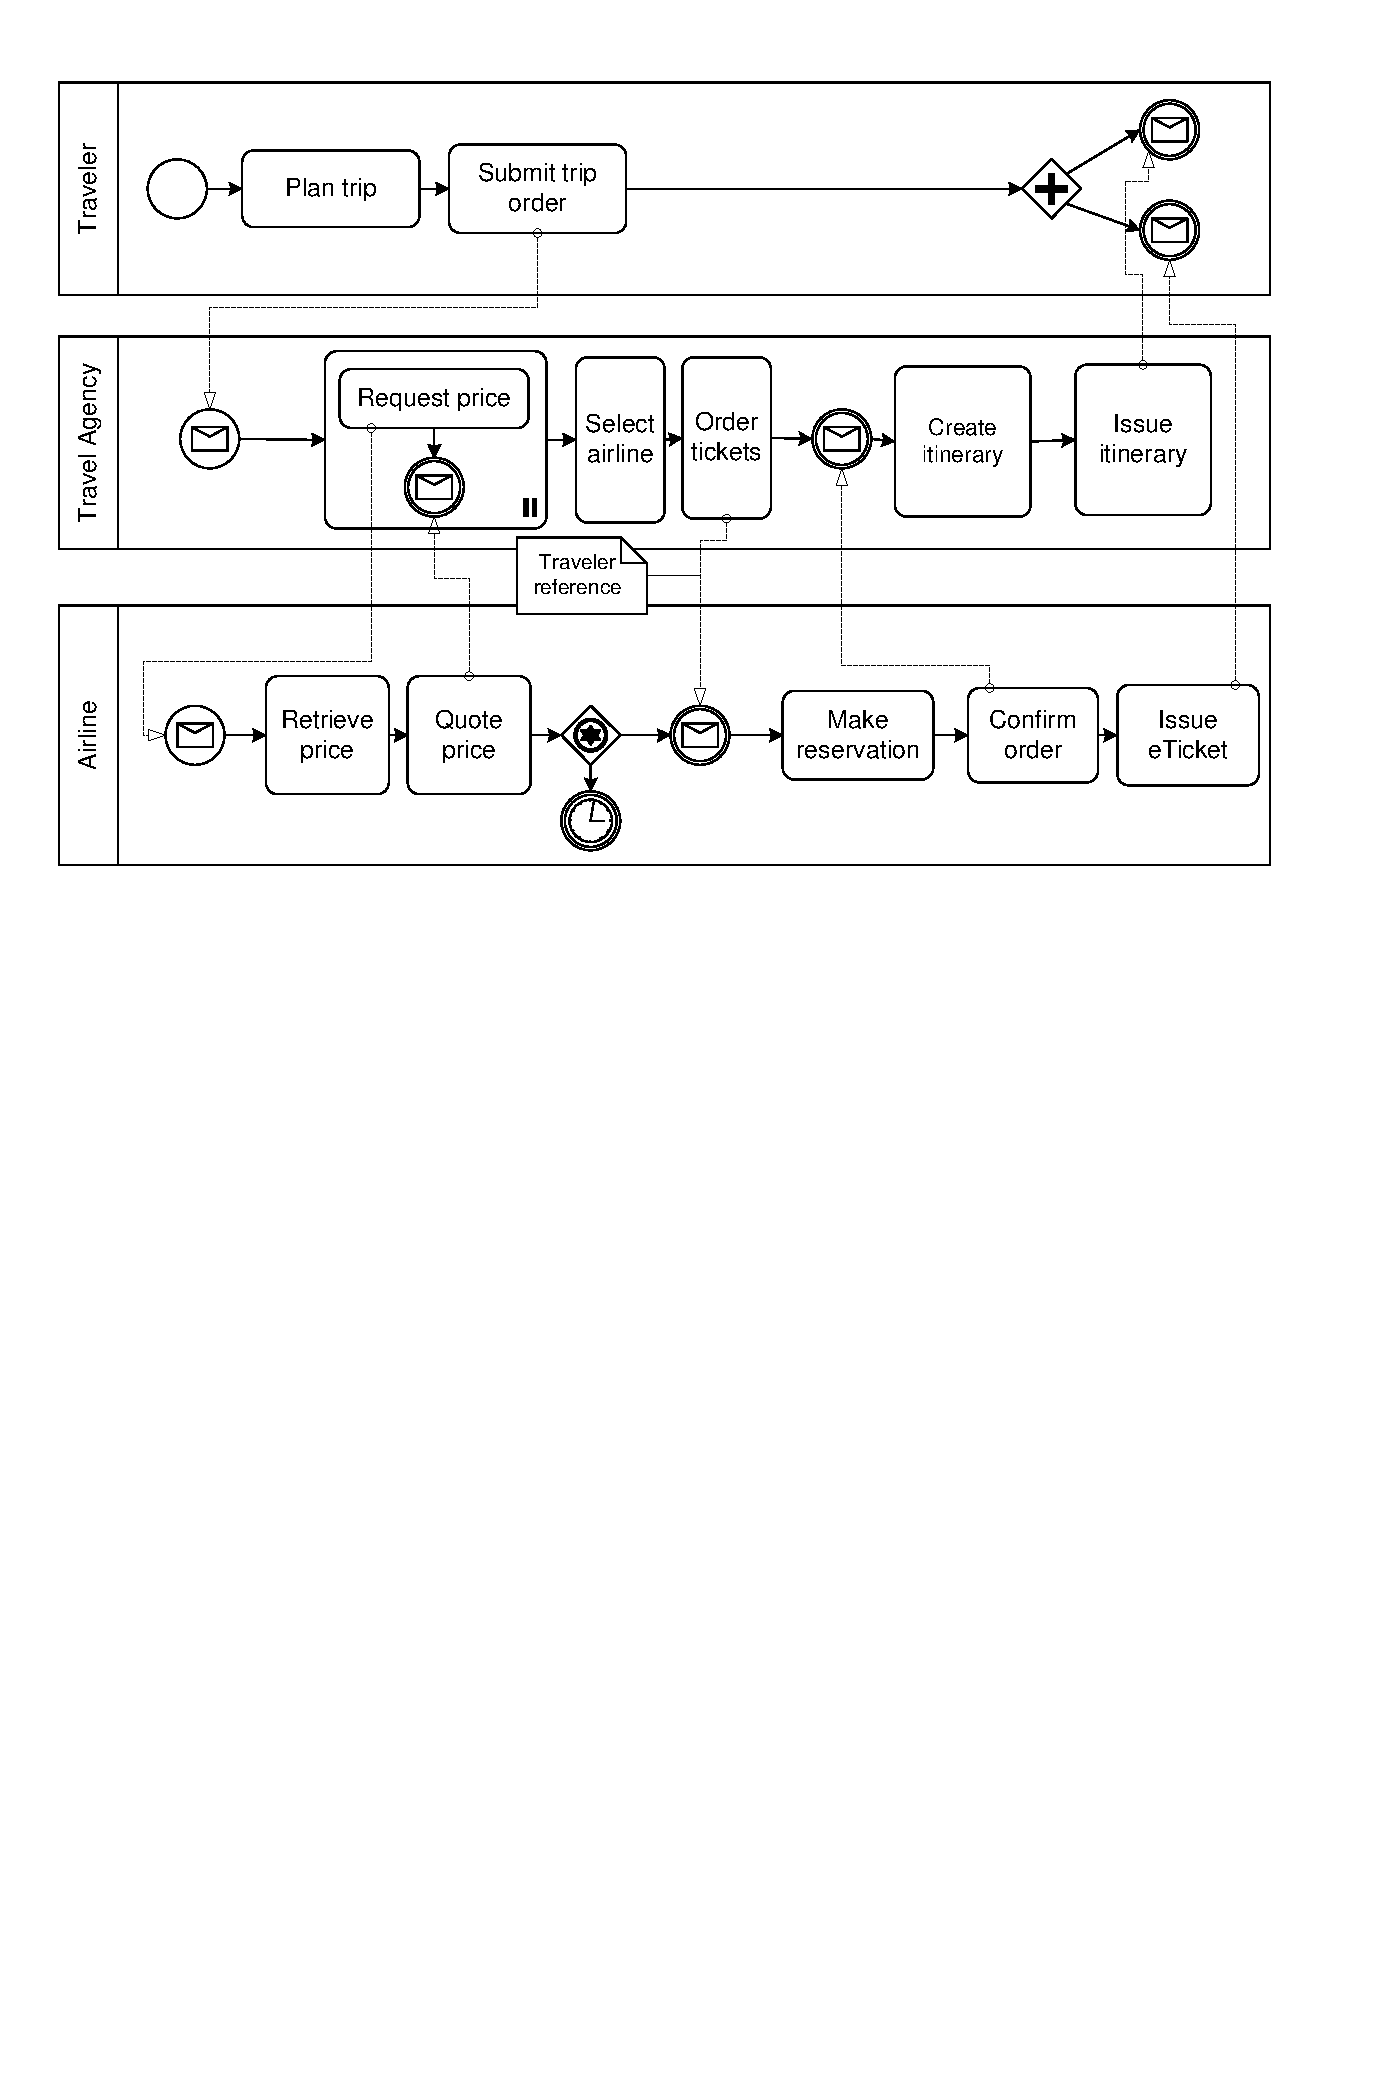
\includegraphics[width=\textwidth]{choreography.pdf}
  \caption{Example Choreography}
  \label{fig:chor1}
\end{figure}

\begin{figure}
  \centering
  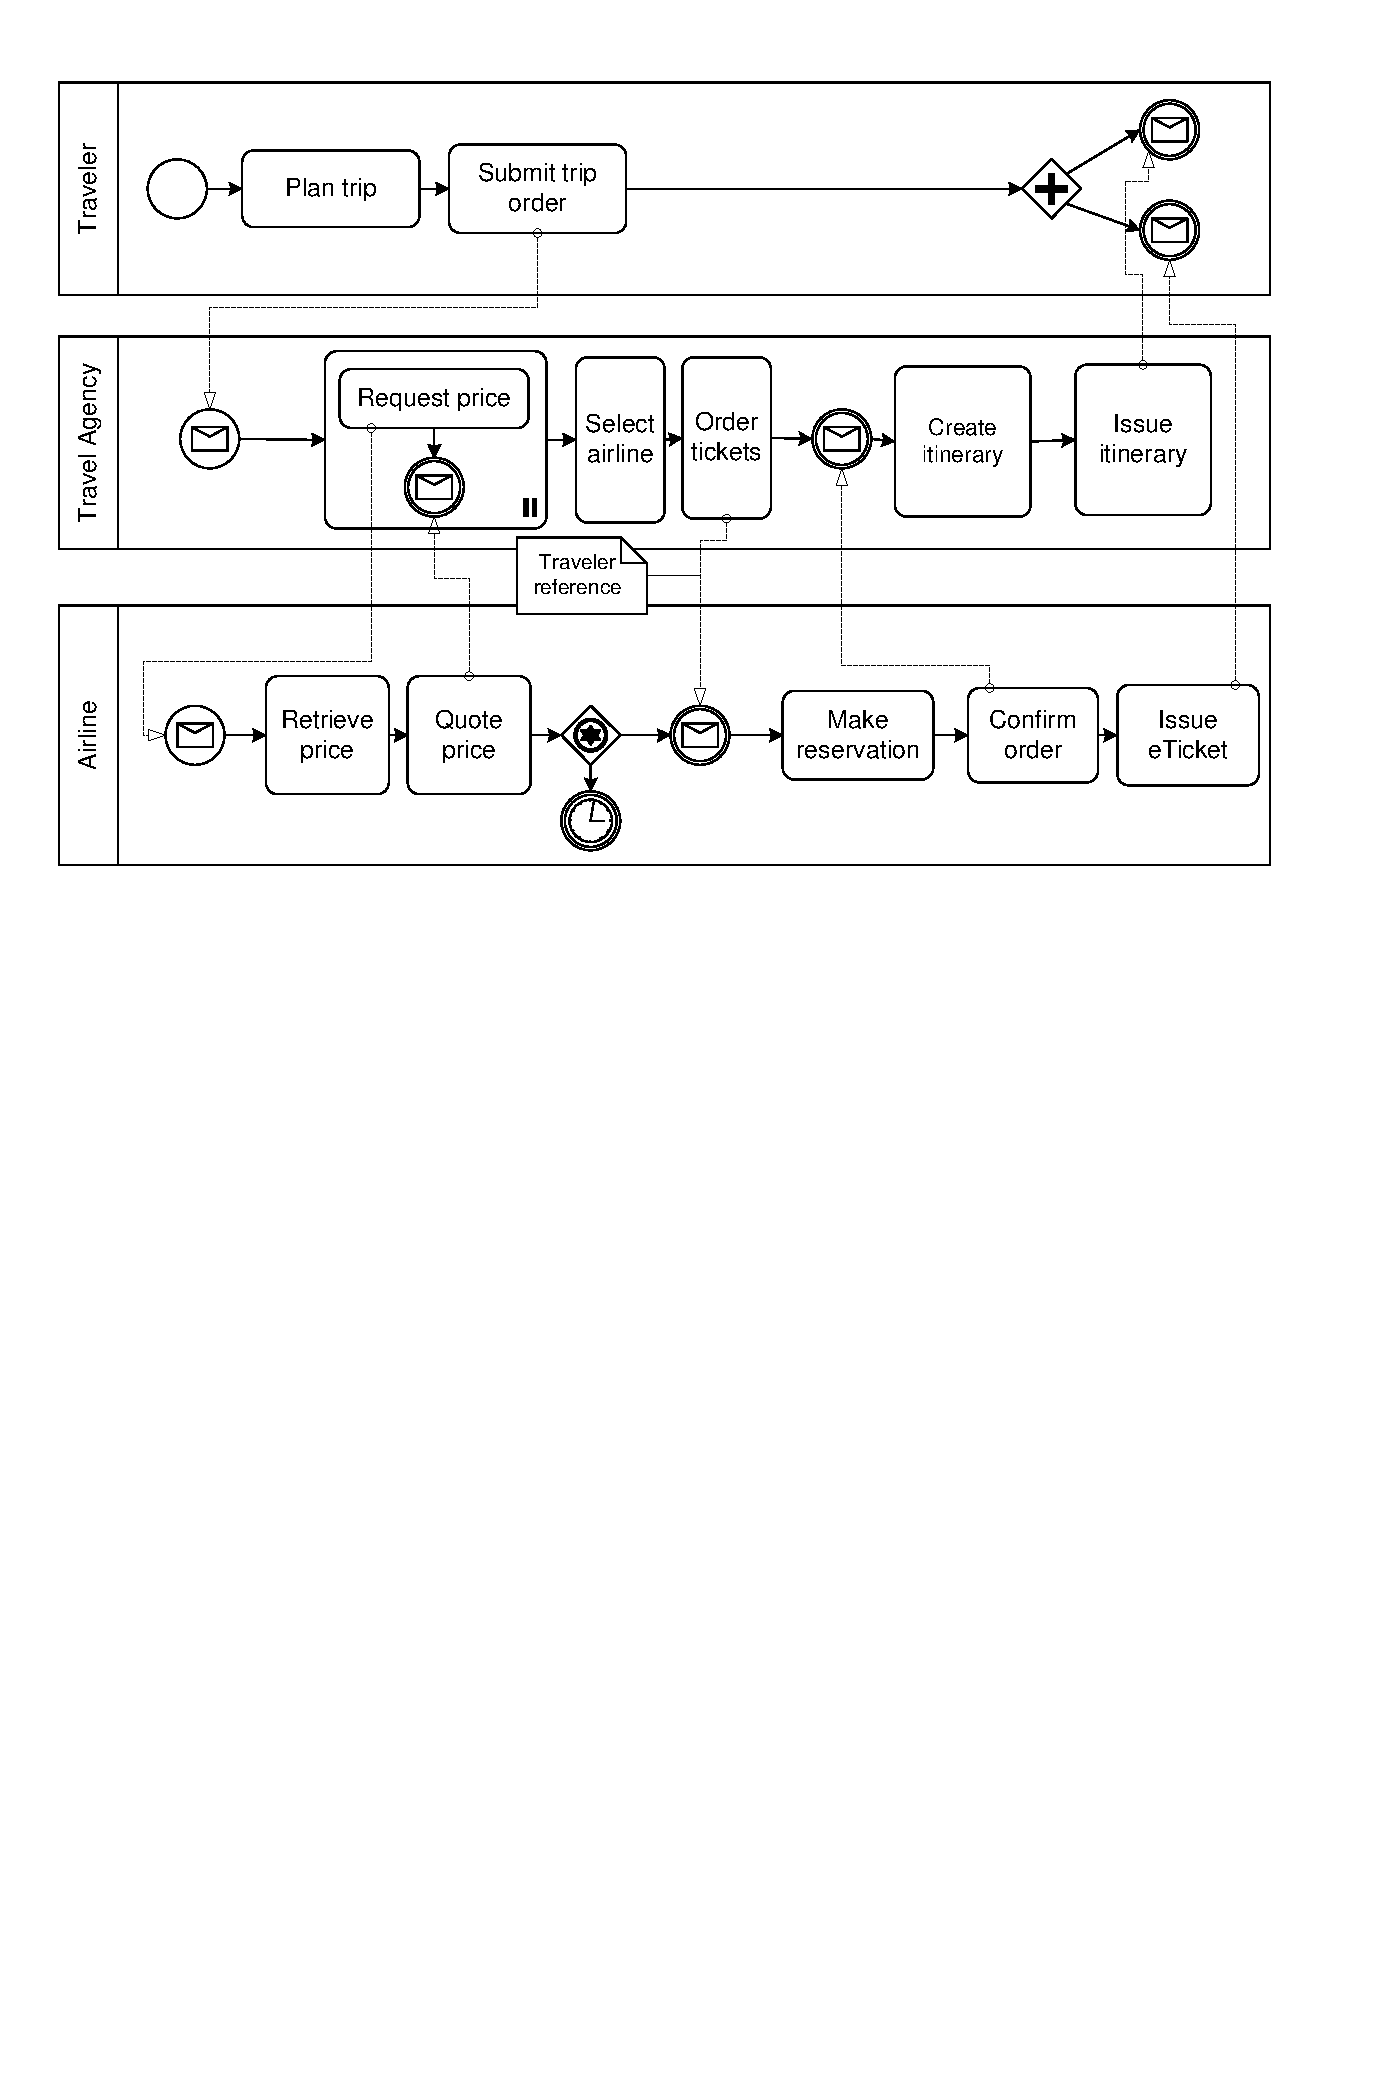
\includegraphics[width=.8\textwidth]{choreography.pdf}
  \caption[Example Choreography]{The example choreography. Now slightly smaller to demonstrate \texttt{\textbackslash textwidth}. And also the use of alternative captions for the list of images. However, the latter is only conditionally recommended, because who reads so much text under a picture? Or is it just a matter of style?}
  \label{fig:chor2}
\end{figure}


\begin{figure}
  \hfill
  \begin{subfigure}{.3\textwidth}
    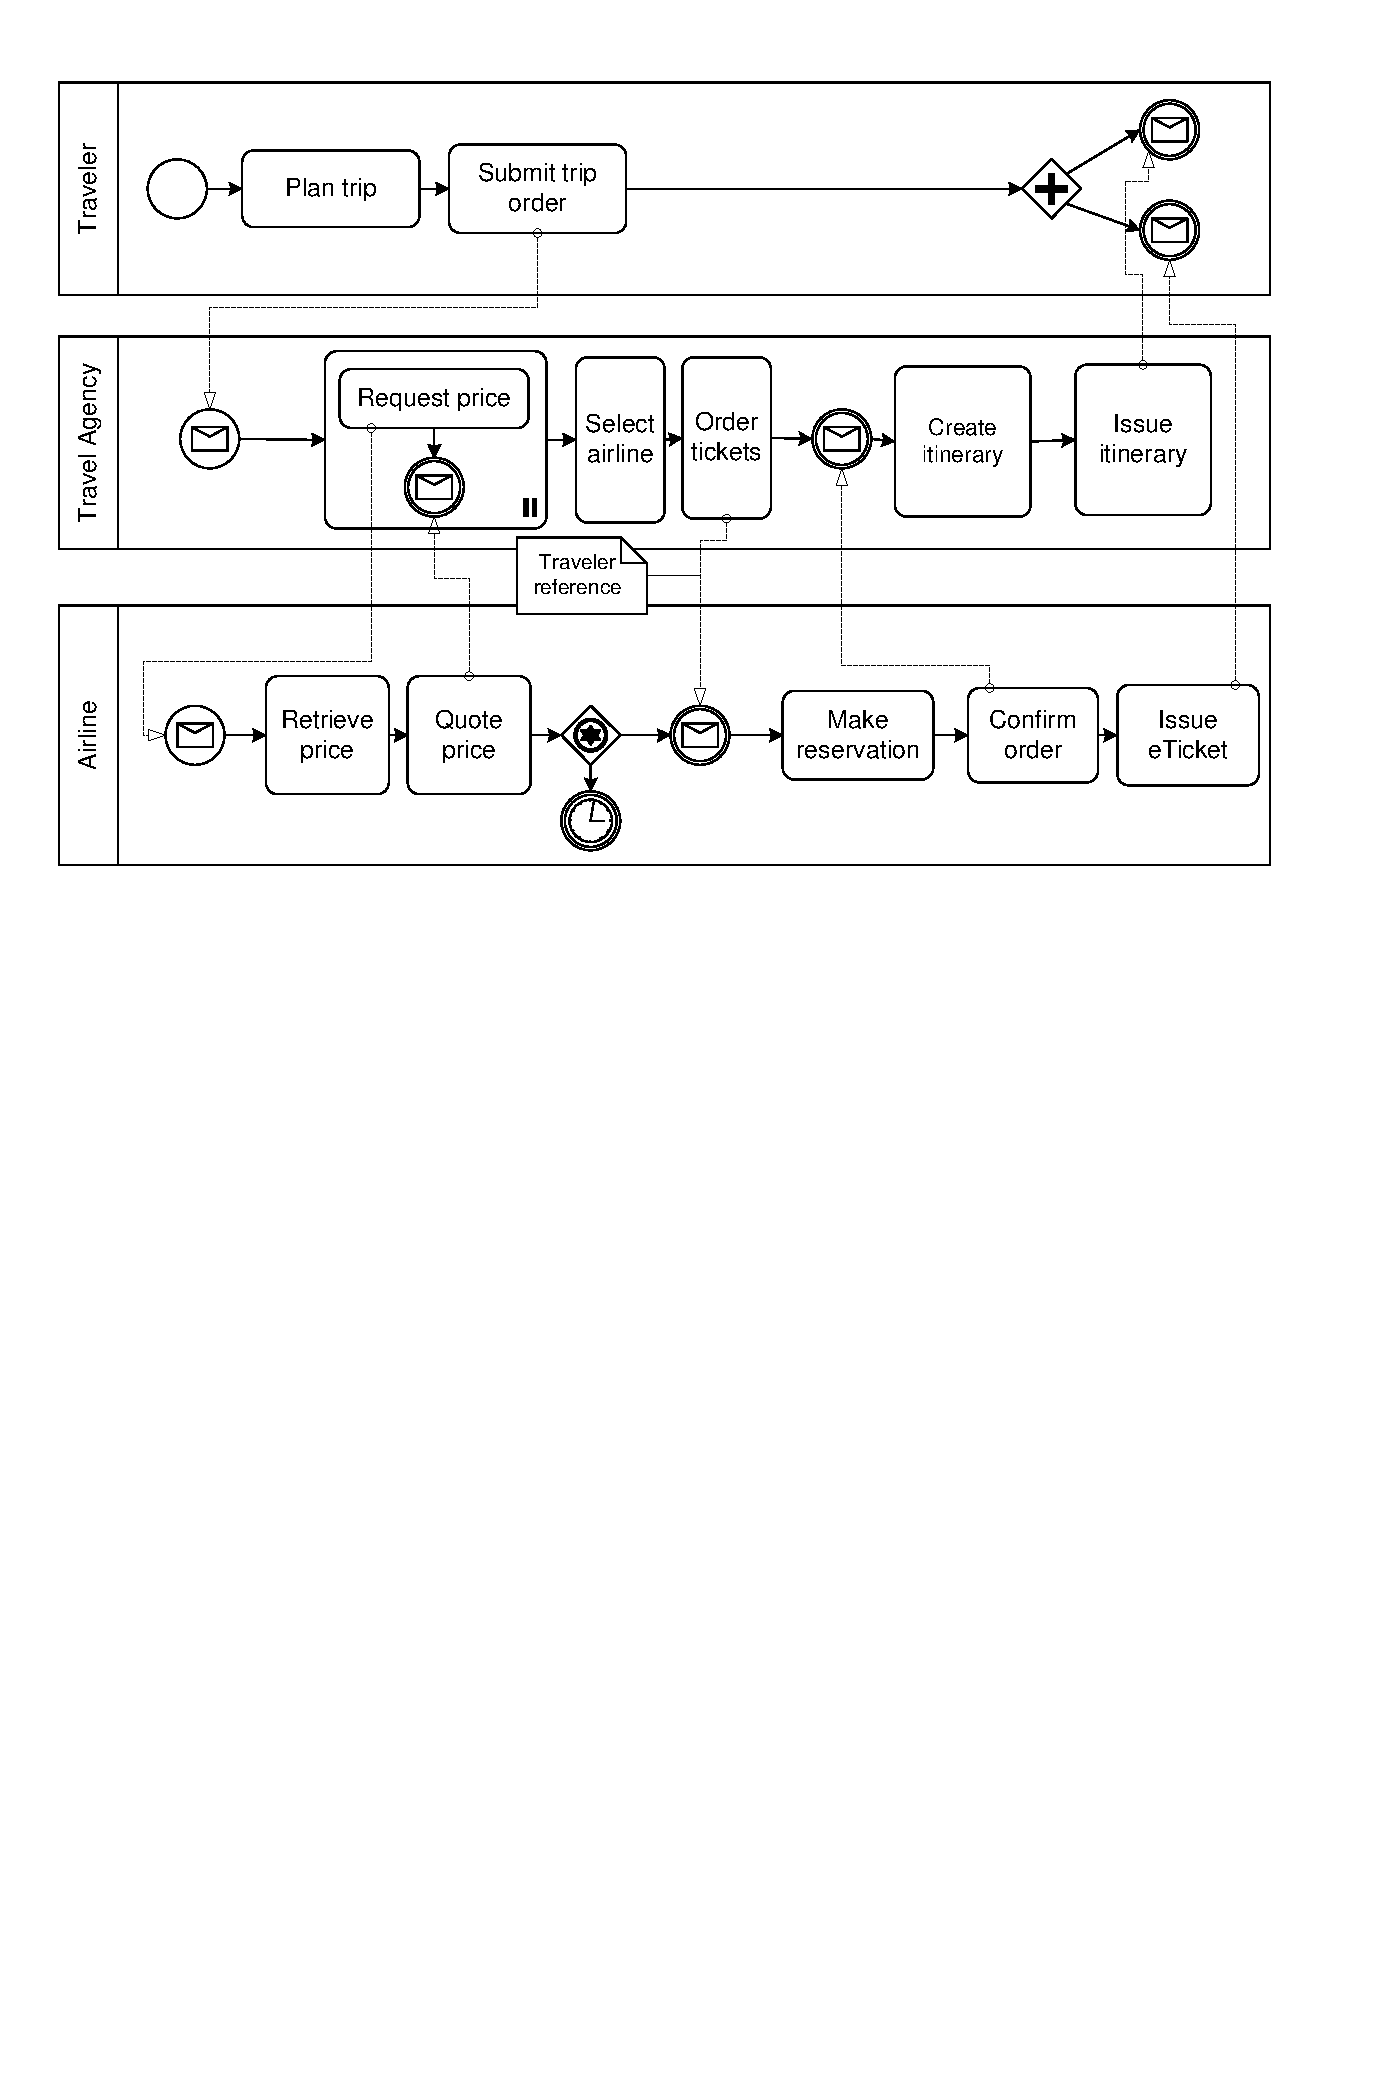
\includegraphics[width=\textwidth]{choreography.pdf}
    \caption{Choreography 1}
    \label{fig:subfigA}
  \end{subfigure}
  \hfill
  \begin{subfigure}{.3\textwidth}
    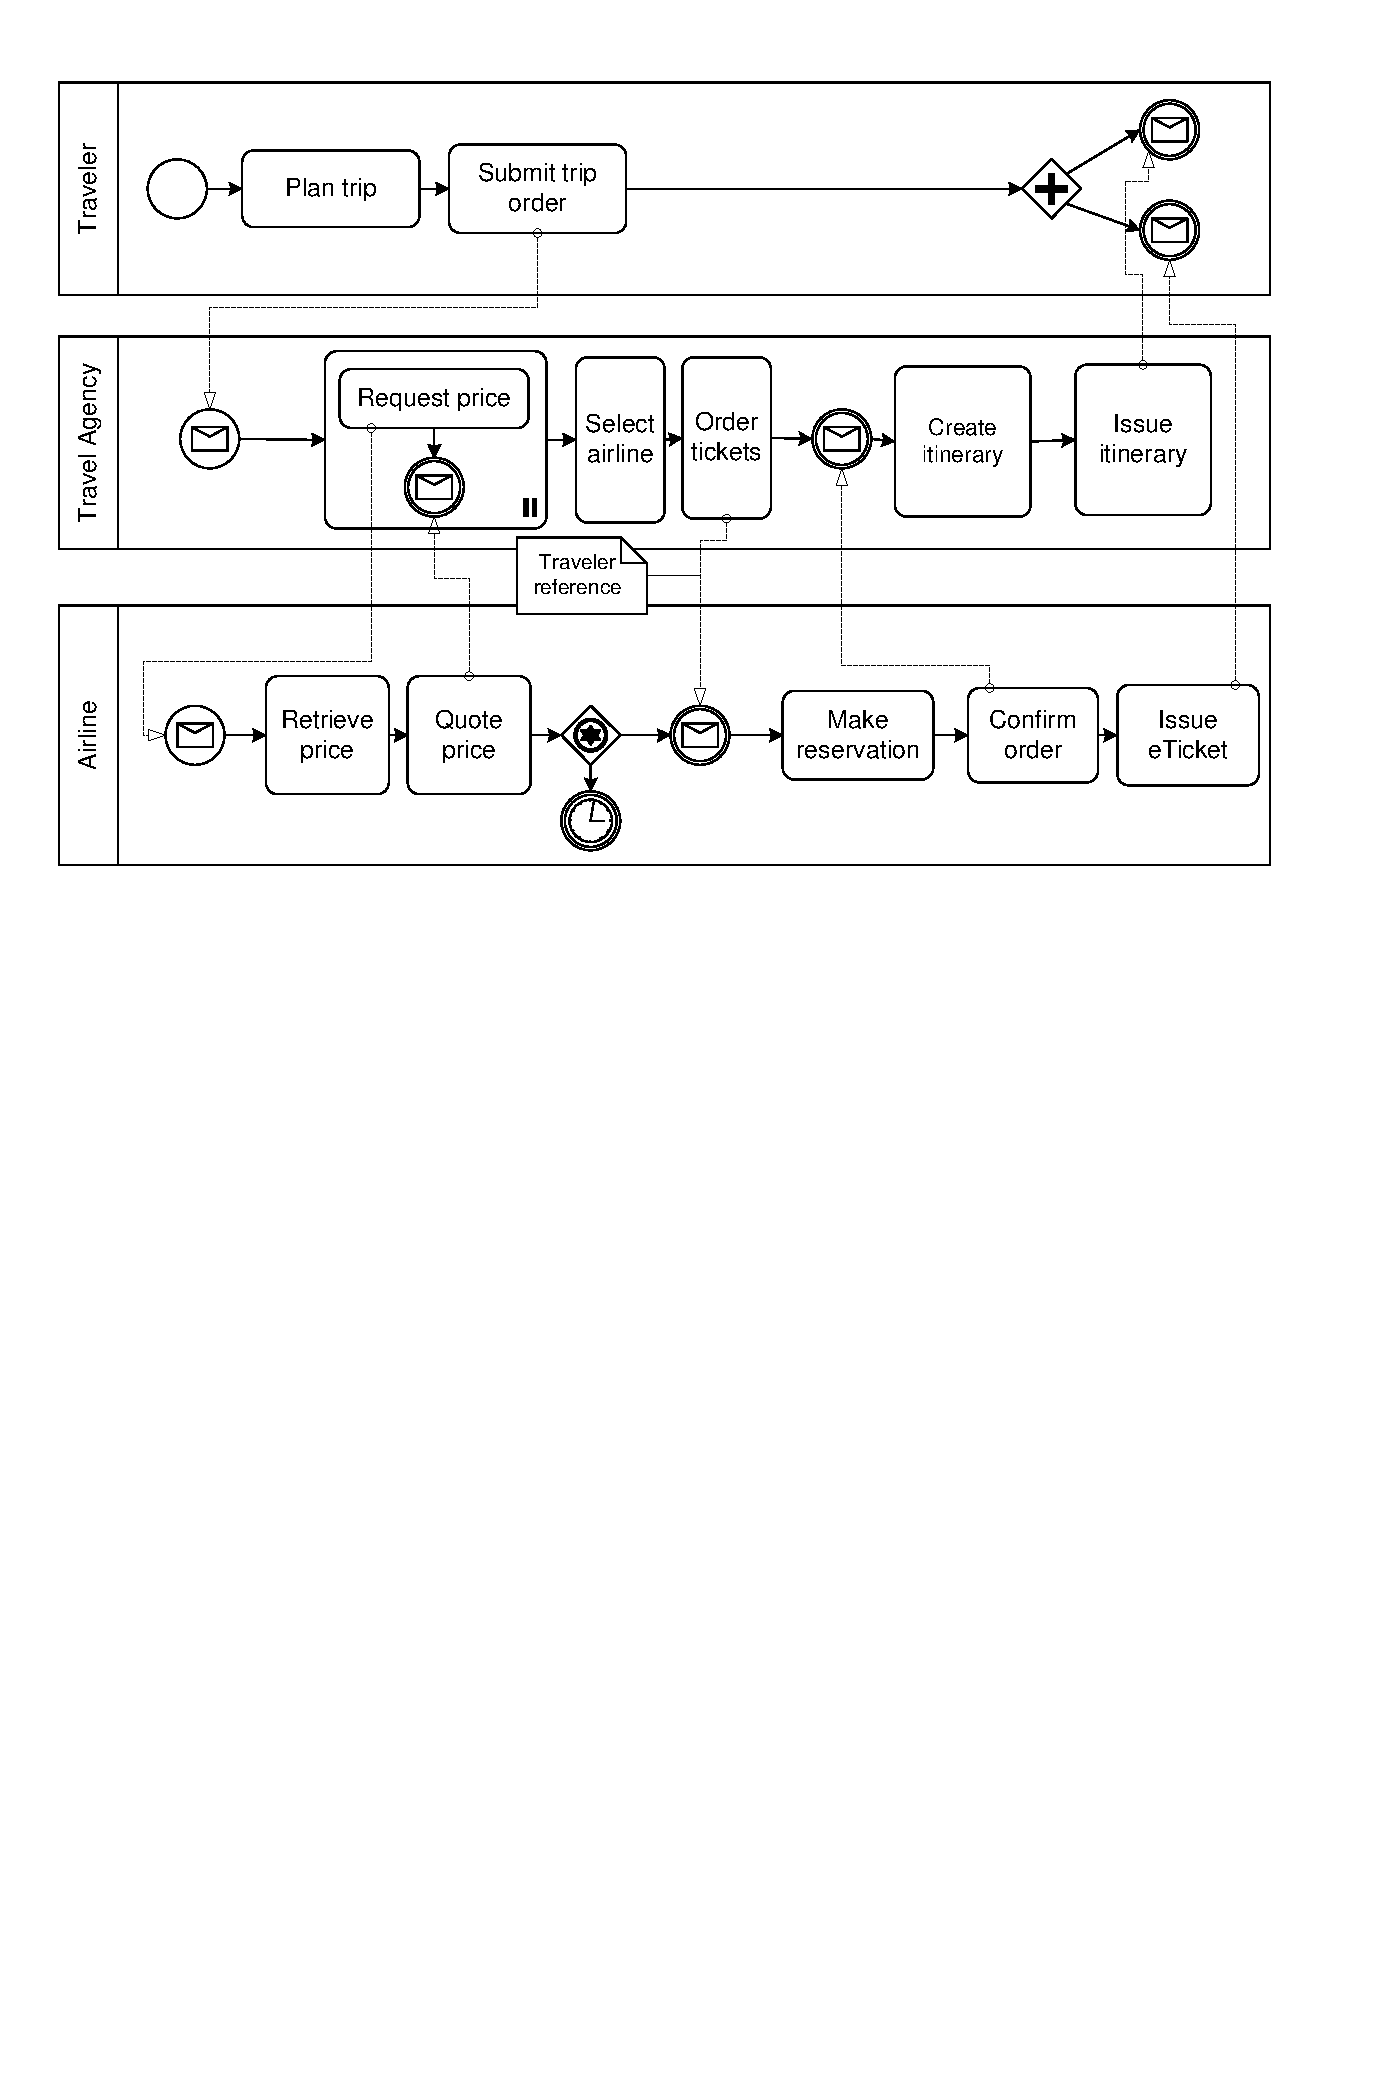
\includegraphics[width=\textwidth]{choreography.pdf}
    \caption{Choreography 2}
    \label{fig:subfigB}
  \end{subfigure}
  \hfill
  \begin{subfigure}{.3\textwidth}
    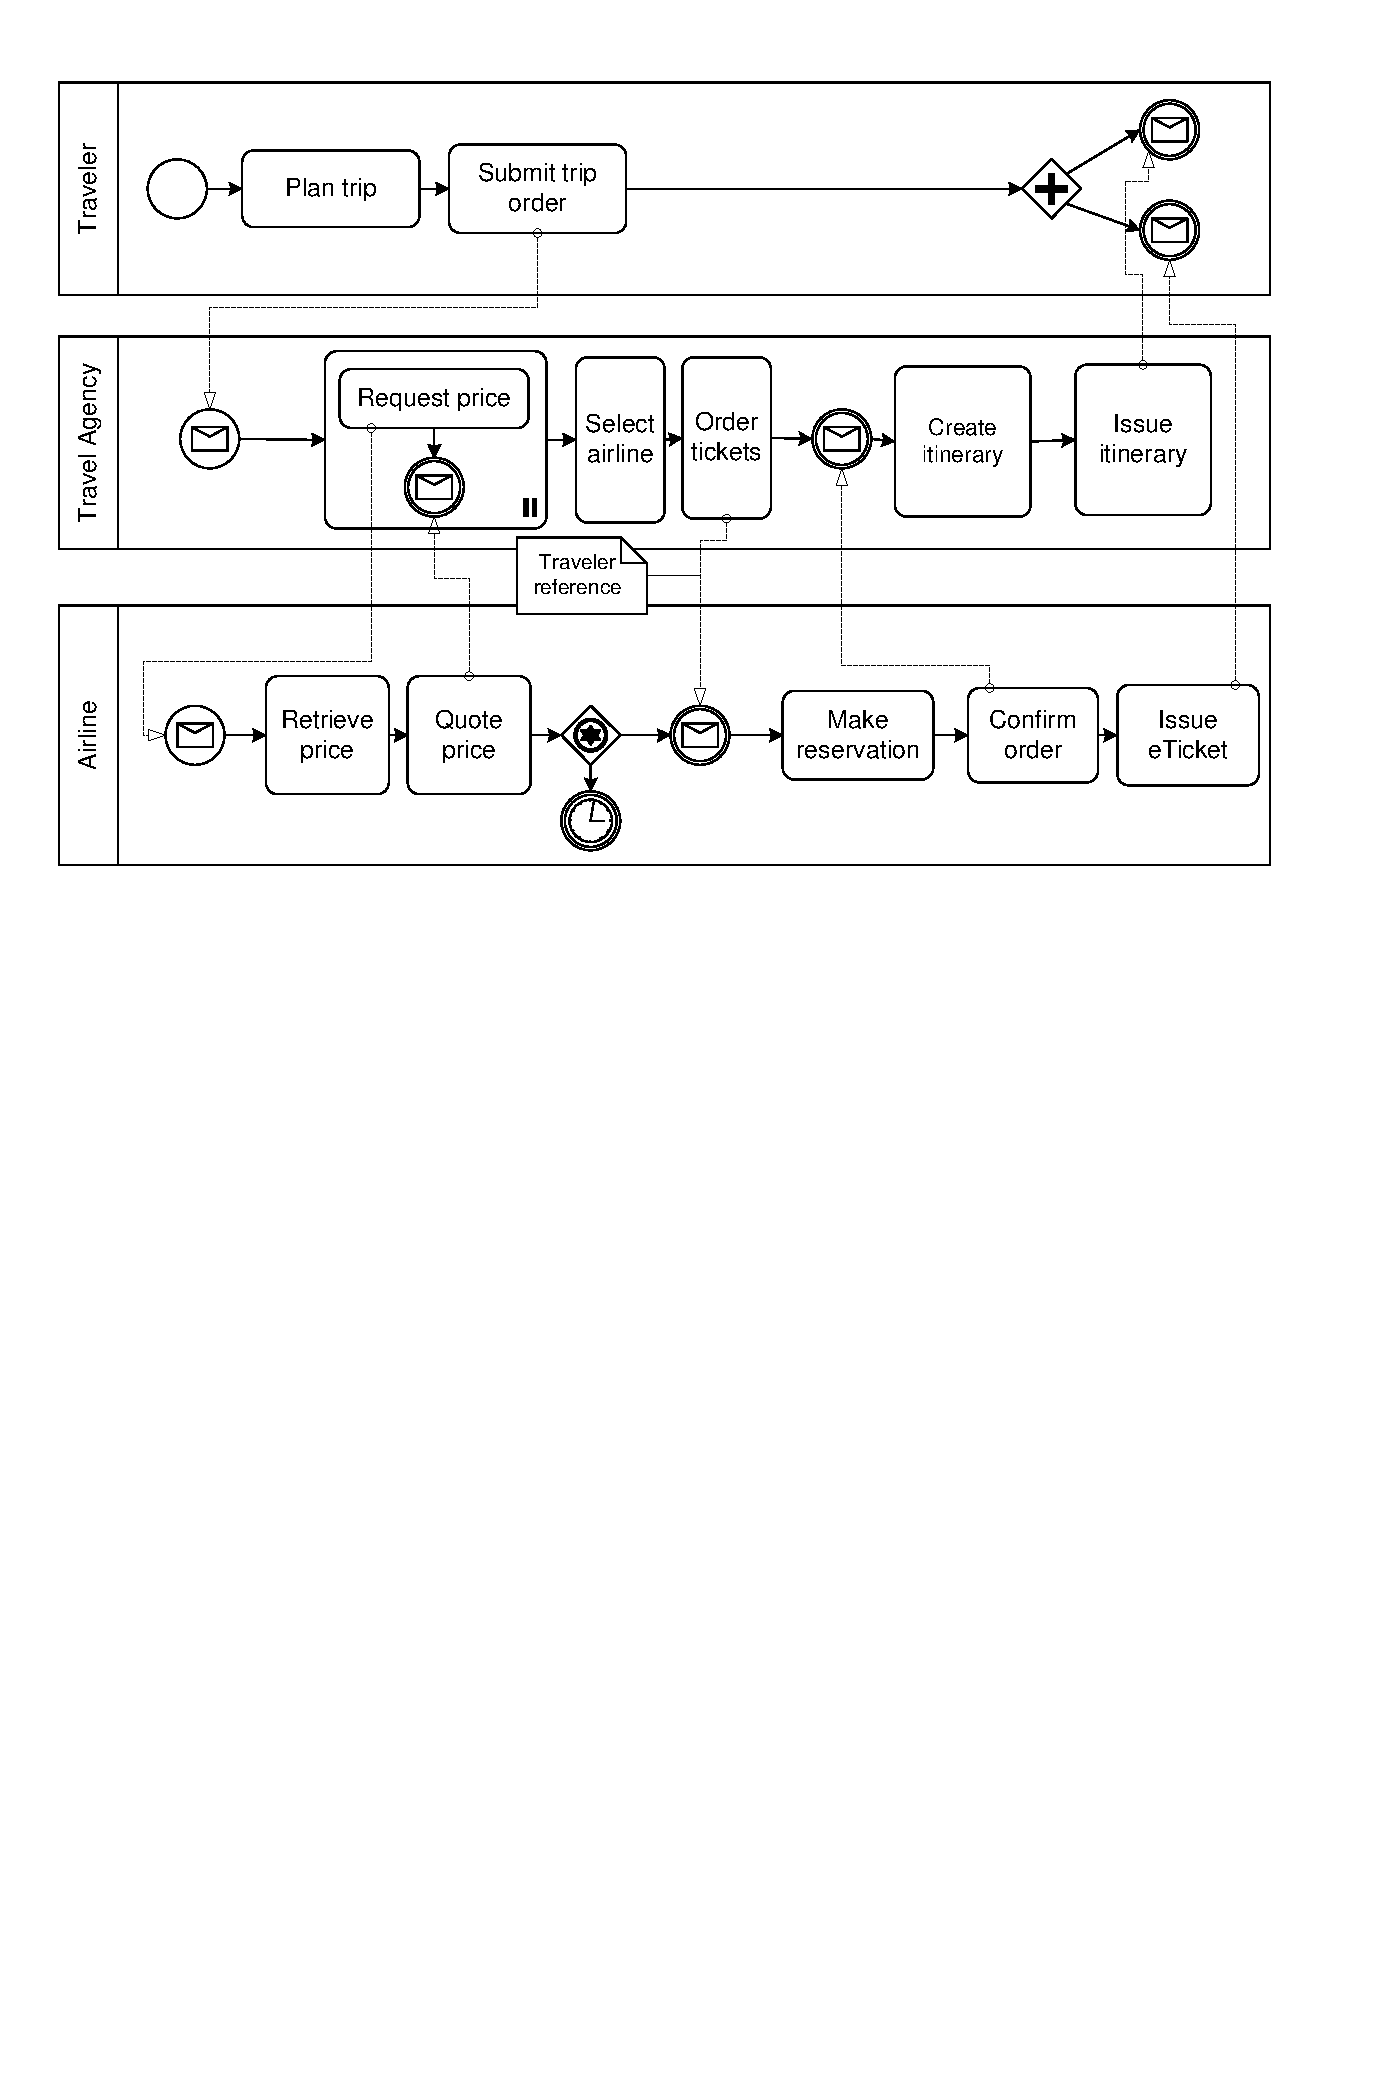
\includegraphics[width=.9\textwidth]{choreography.pdf}
    \caption{Choreography 3}
    \label{fig:subfigC}
  \end{subfigure}
  \caption{Example to place 3 illustrations next to each other. Further, it is possible to reference each separately.}
  \label{fig:subfig_example}
\end{figure}

\Cref{fig:subfig_example} shows the usage of the package subcaption.
It is indeed possible to reference to sub figures: \Cref{fig:subfigA}.

It is possible to convert SVGs to PDF directly during compilation.
This is described in the source code of latex-tipps.tex, but commented out.

\iffalse % <-- Take this away if inkscape is in the path
  The SVG in \cref{fig:directSVG} is directly included, while the text in the SVG in \cref{fig:latexSVG} is set using pdflatex.
  If you want to see the graphics, inkscape must be in PATH and in the text source \texttt{\textbackslash{}iffalse} and \text{\textbackslash{}iftrue} have to be commented out.

  \begin{figure}
    \centering
    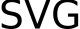
\includegraphics{svgexample.svg}
    \caption{SVG directly included}
    \label{fig:directSVG}
  \end{figure}

  \begin{figure}
    \centering
    \def\svgwidth{.4\textwidth}
    \includesvg{svgexample}
    \caption{Text in SVN set via \LaTeX{}}
    \label{fig:latexSVG}
  \end{figure}
\fi % <-- Take this away if inkscape is in the path



\section{More Illustrations}
\Cref{fig:AnhangsChor,fig:AnhangsChor2} show two choreographies, which should further explain the facts. The second figure is rotated 90 degrees to demonstrate the \texttt{pdflscape} package.

\begin{figure}
  \centering
  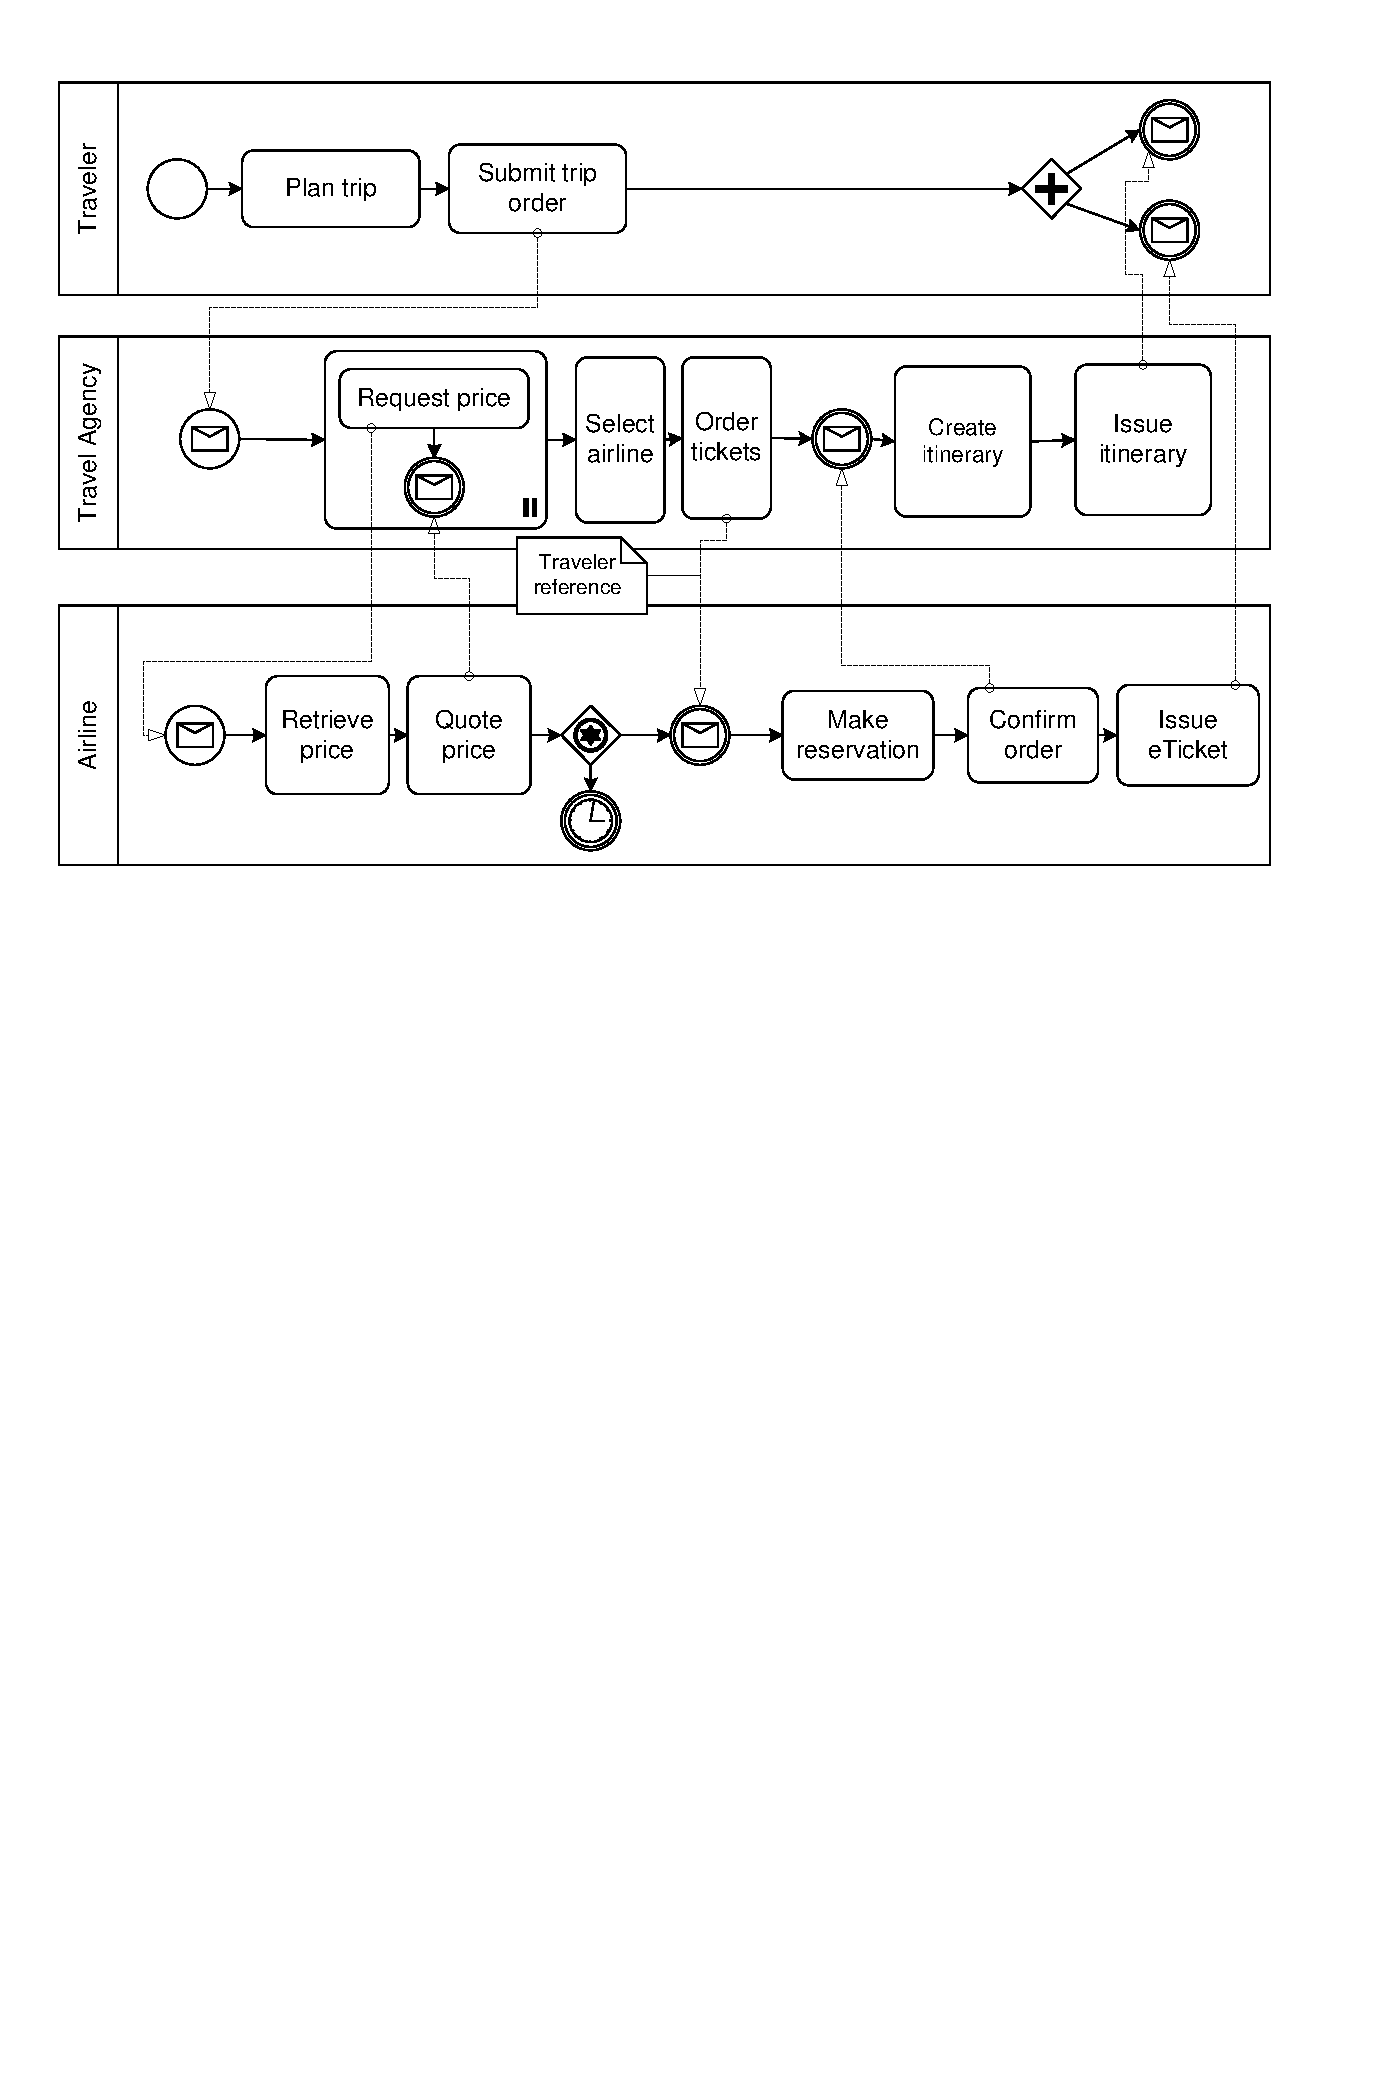
\includegraphics[width=\textwidth]{choreography.pdf}
  \caption{Example Choreography I}
  \label{fig:AnhangsChor}
\end{figure}

\begin{landscape}
  %sidewaysfigure
  \begin{figure}
    \centering
    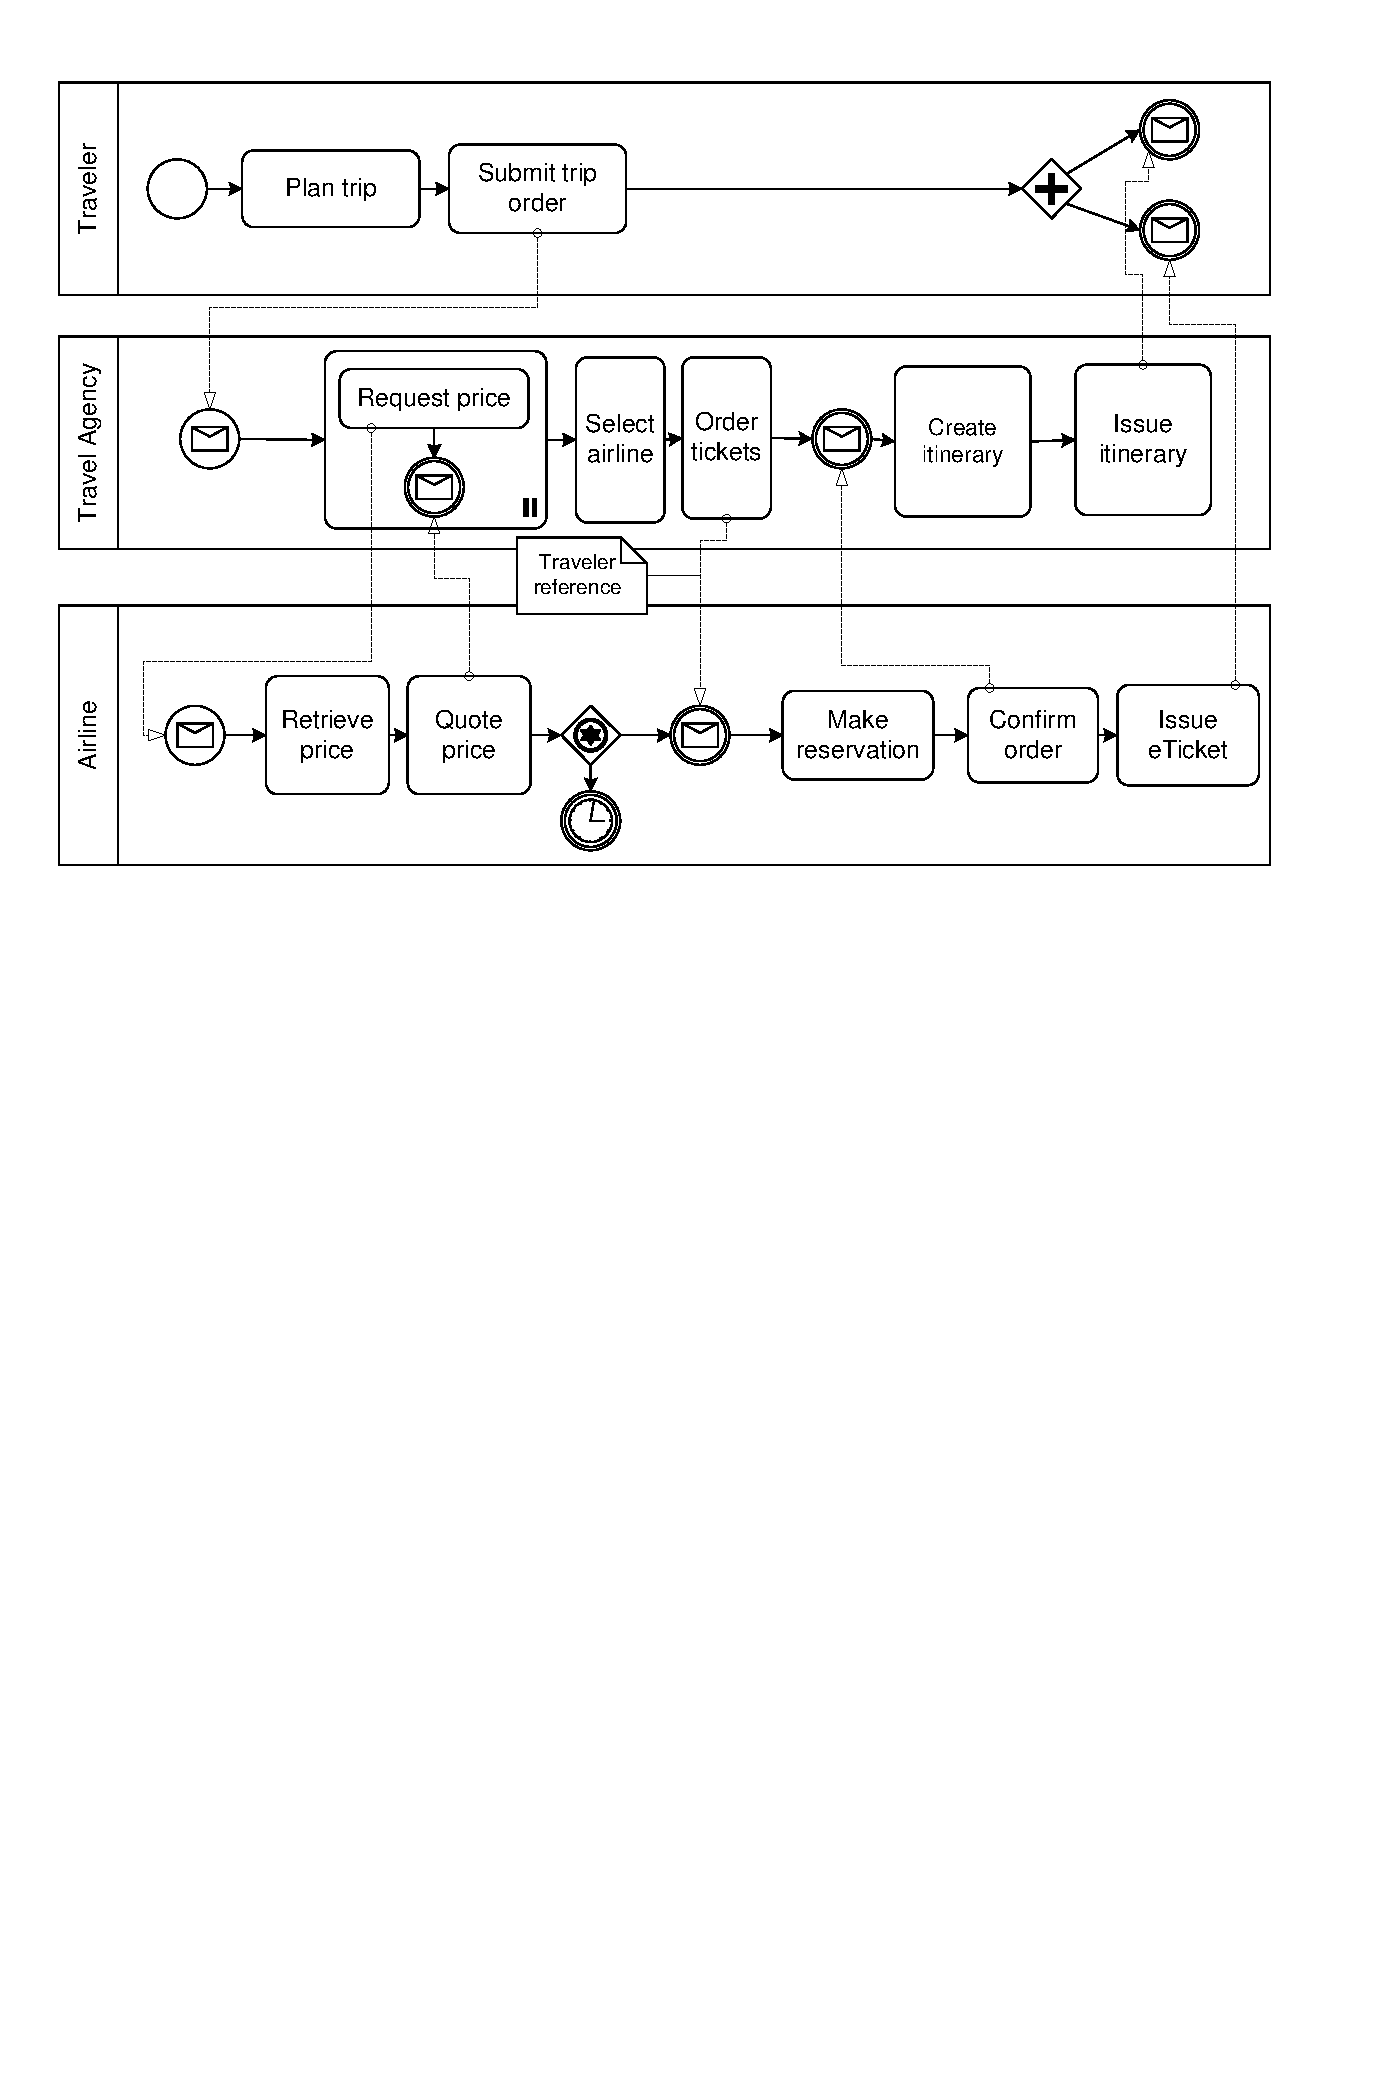
\includegraphics[width=\textwidth]{choreography.pdf}
    \caption{Example Choreography II}
    \label{fig:AnhangsChor2}
  \end{figure}
\end{landscape}


\IfFileExists{pgfplots.sty}{
  %%%%%%%%%%%%%%%%%%%%%%%%%%%%%%%%%%%%%%%%%%%%%%%%%%%%%%%%%%%%%%%%%%%%%%%%%%%%%%
  \section{Plots with pgfplots}
  %%%%%%%%%%%%%%%%%%%%%%%%%%%%%%%%%%%%%%%%%%%%%%%%%%%%%%%%%%%%%%%%%%%%%%%%%%%%%%
  The package pdfplots provides plotting of functions directly in \LaTeX~like with matlab or gnuplot. Some visual examples are available here\footnote{\url{http://texdoc.net/pkg/visualtikz}}.
  \begin{figure}[h]
    \begin{center}
      \begin{tikzpicture}
        \begin{axis}[xlabel=$x$,
            ylabel=$\sin(x)$]
          \addplot {sin(deg(x))};  % Print sine function
        \end{axis}
      \end{tikzpicture}
    \end{center}
    \caption{Plot of $\sin(x)$ direclty inside the figure environment with pgfplots.}
  \end{figure}

  \begin{figure}[h]
    \begin{center}
      \begin{tikzpicture}
        \begin{axis}[xlabel=$x$,
            ylabel=$y$]
          \addplot table [x=a, y=c, col sep=comma] {data/data.csv};  % Read coordinates from csv file and plot them
        \end{axis}
      \end{tikzpicture}
    \end{center}
    \caption{Coordinates $x$ and $y$ read from csv file and plotted pgfplots.}
  \end{figure}

}{}


%%%%%%%%%%%%%%%%%%%%%%%%%%%%%%%%%%%%%%%%%%%%%%%%%%%%%%%%%%%%%%%%%%%%%%%%%%%%%%
\section{Figures with tikz}
%%%%%%%%%%%%%%%%%%%%%%%%%%%%%%%%%%%%%%%%%%%%%%%%%%%%%%%%%%%%%%%%%%%%%%%%%%%%%%
The tikz is a package for creating graphics programmatically. With this package grids or other regular strucutres can be easliy generated.

\begin{figure}[ht]
  \begin{center}
    \begin{tikzpicture}
      \draw(0,0) rectangle (4,4);
      \foreach \x in {0.5,1,1.5,2,2.5,3,3.5}
      \foreach \y in {0.5,1,1.5,2,2.5,3,3.5}
      \draw(\x,\y) circle (1pt);
    \end{tikzpicture}
  \end{center}
  \caption{A regular grid genrated with easily with two for loops.}\label{fig:tikz_example}
\end{figure}


%%%%%%%%%%%%%%%%%%%%%%%%%%%%%%%%%%%%%%%%%%%%%%%%%%%%%%%%%%%%%%%%%%%%%%%%%%%%%%
\section{UML diagrams using tikz-uml}
%%%%%%%%%%%%%%%%%%%%%%%%%%%%%%%%%%%%%%%%%%%%%%%%%%%%%%%%%%%%%%%%%%%%%%%%%%%%%%

\Cref{fig:uml} presents a class diagram typeset using tikz-uml.

\begin{center}
\begin{figure}
\begin{tikzpicture}
\begin{umlpackage}{p}
\begin{umlpackage}{sp1}
\umlclass[template=T]{A}{
  n : uint \\ t : float
}{}
\umlclass[y=-3]{B}{
  d : double
}{
  \umlvirt{setB(b : B) : void} \\ getB() : B}
\end{umlpackage}
\begin{umlpackage}[x=10,y=-6]{sp2}
\umlinterface{C}{
  n : uint \\ s : string
}{}
\end{umlpackage}
\umlclass[x=2,y=-10]{D}{
  n : uint
  }{}
\end{umlpackage}

\umlassoc[geometry=-|-, arg1=tata, mult1=*, pos1=0.3, arg2=toto, mult2=1, pos2=2.9, align2=left]{C}{B}
\umlunicompo[geometry=-|, arg=titi, mult=*, pos=1.7, stereo=vector]{D}{C}
\umlimport[geometry=|-, anchors=90 and 50, name=import]{sp2}{sp1}
\umlaggreg[arg=tutu, mult=1, pos=0.8, angle1=30, angle2=60, loopsize=2cm]{D}{D}
\umlinherit[geometry=-|]{D}{B}
\umlnote[x=2.5,y=-6, width=3cm]{B}{A note with respect to class B}
\umlnote[x=7.5,y=-2]{import-2}{A anotation}
\end{tikzpicture}
\caption{Class diagram generated with tikz-uml. Example adapted from Nicolas Kielbasiewicz.}
\label{fig:uml}
\end{figure}
\end{center}

\section{UML diagrams using PlantUML}

In case \lualatex{} is used and PlantUML is installed, UML diagrams can be defined using PlantUML.

% Only works if "--shell-escape" is activated. Please activate only if you are sure, your compilation settings are correct
%\IfFileExists{plantuml.sty}{\input{latexhints-english-plantuml}}{}

%%%%%%%%%%%%%%%%%%%%%%%%%%%%%%%%%%%%%%%%%%%%%%%%%%%%%%%%%%%%%%%%%%%%%%%%%%%%%%
\section{Tables}
%%%%%%%%%%%%%%%%%%%%%%%%%%%%%%%%%%%%%%%%%%%%%%%%%%%%%%%%%%%%%%%%%%%%%%%%%%%%%%
\cref{tab:Ergebnisse} shows results and \cref{tab:Results} shows how numerical data can be represented in a table.
\begin{table}
  \centering
  \begin{tabular}{ccc}
    \toprule
    \multicolumn{2}{c}{\textbf{summed}} & \textbf{Title}                                                          \\ \midrule
    Table                                      & as                                                           & in      \\
    \url{tabsatz.pdf}                            & recommended                                                     & gesetzt \\

    \multirow{2}{*}{Example}                    & \multicolumn{2}{c}{a nice example}                                \\
                                                 & \multicolumn{2}{c}{for using \qq{multirow}}           \\
    \bottomrule
  \end{tabular}
  \caption[Example Table]{Exampe Table -- see \url{http://www.ctan.org/tex-archive/info/german/tabsatz/}}
  \label{tab:Ergebnisse}
\end{table}

\begin{table}
  \centering
  \begin{tabular}{l *{8}{d{3.2}}}
    \toprule

                         & \multicolumn{2}{c}{\textbf{Parameter 1}} & \multicolumn{2}{c}{\textbf{Parameter 2}} & \multicolumn{2}{c}{\textbf{Parameter 3}} & \multicolumn{2}{c}{\textbf{Parameter 4}}                                                                                                                                       \\
    \cmidrule(r){2-3}\cmidrule(lr){4-5}\cmidrule(lr){6-7}\cmidrule(l){8-9}

    \textbf{Bedingungen} & \multicolumn{1}{c}{\textbf{M}}           & \multicolumn{1}{c}{\textbf{SD}}          & \multicolumn{1}{c}{\textbf{M}}           & \multicolumn{1}{c}{\textbf{SD}}          & \multicolumn{1}{c}{\textbf{M}} & \multicolumn{1}{c}{\textbf{SD}} & \multicolumn{1}{c}{\textbf{M}} & \multicolumn{1}{c}{\textbf{SD}} \\
    \midrule

    W                    & 1.1                                      & 5.55                                     & 6.66                                     & .01                                      &                                &                                 &                                &                                 \\
    X                    & 22.22                                    & 0.0                                      & 77.5                                     & .1                                       &                                &                                 &                                &                                 \\
    Y                    & 333.3                                    & .1                                       & 11.11                                    & .05                                      &                                &                                 &                                &                                 \\
    Z                    & 4444.44                                  & 77.77                                    & 14.06                                    & .3                                       &                                &                                 &                                &                                 \\
    \bottomrule
  \end{tabular}

  \caption{Example table for 4 constraints (W-Z), each having 4 parameters with (M und SD). Note: use always the same number of decimal places.}
  \label{tab:Werte}
\end{table}

\IfFileExists{pgfplotstable.sty}{

\subsection{Tables with pgfplots}
With the pgfplotstable package tables can be directly generated from a csv file.

\begin{table}[h]
\centering
\pgfplotstabletypeset[
col sep = comma,
every head row/.style={before row=\toprule,after row=\midrule},
every last row/.style={after row=\bottomrule},
display columns/0/.style={string type,column name={}}
]
{data/data.csv}
\caption{Table direclty generated from the values of a csf file.}
\end{table}
}{}


\section{Tables spanning multiple pages}


\begin{longtable}{|l|l|l|}
\caption{A sample long table.} \label{tab:long} \\

\hline \multicolumn{1}{|c|}{\textbf{First column}} & \multicolumn{1}{c|}{\textbf{Second column}} & \multicolumn{1}{c|}{\textbf{Third column}} \\ \hline
\endfirsthead

\multicolumn{3}{c}%
{{\bfseries \tablename\ \thetable{} -- continued from previous page}} \\
\hline \multicolumn{1}{|c|}{\textbf{First column}} & \multicolumn{1}{c|}{\textbf{Second column}} & \multicolumn{1}{c|}{\textbf{Third column}} \\ \hline
\endhead

\hline \multicolumn{3}{|r|}{{Continued on next page}} \\ \hline
\endfoot

\hline \hline
\endlastfoot

A & BC & D \\
A & BC & D \\
A & BC & D \\
A & BC & D \\
A & BC & D \\
A & BC & D \\
A & BC & D \\
A & BC & D \\
A & BC & D \\
A & BC & D \\
A & BC & D \\
A & BC & D \\
A & BC & D \\
A & BC & D \\
A & BC & D \\
A & BC & D \\
A & BC & D \\
A & BC & D \\
A & BC & D \\
A & BC & D \\
A & BC & D \\
A & BC & D \\
A & BC & D \\
A & BC & D \\
A & BC & D \\
A & BC & D \\
A & BC & D \\
A & BC & D \\
A & BC & D \\
A & BC & D \\
A & BC & D \\
A & BC & D \\
A & BC & D \\
A & BC & D \\
A & BC & D \\
A & BC & D \\
A & BC & D \\
A & BC & D \\
A & BC & D \\
A & BC & D \\
A & BC & D \\
A & BC & D \\
A & BC & D \\
A & BC & D \\
A & BC & D \\
A & BC & D \\
A & BC & D \\
A & BC & D \\
A & BC & D \\
A & BC & D \\
A & BC & D \\
A & BC & D \\
A & BC & D \\
A & BC & D \\
A & BC & D \\
A & BC & D \\
A & BC & D \\
A & BC & D \\
A & BC & D \\
A & BC & D \\
A & BC & D \\
A & BC & D \\
A & BC & D \\
A & BC & D \\
A & BC & D \\
A & BC & D \\
A & BC & D \\
A & BC & D \\
A & BC & D \\
A & BC & D \\
A & BC & D \\
A & BC & D \\
A & BC & D \\
A & BC & D \\
A & BC & D \\
A & BC & D \\
A & BC & D \\
A & BC & D \\
A & BC & D \\
A & BC & D \\
\end{longtable}


%%%%%%%%%%%%%%%%%%%%%%%%%%%%%%%%%%%%%%%%%%%%%%%%%%%%%%%%%%%%%%%%%%%%%%%%%%%%%%
\section{Abbreviations}
%%%%%%%%%%%%%%%%%%%%%%%%%%%%%%%%%%%%%%%%%%%%%%%%%%%%%%%%%%%%%%%%%%%%%%%%%%%%%%
At the first pass the \gls{fr} was 5.
At the second pass was \gls{fr} 3.
The plural form can be seen here: \glspl{er}.
To demonstrate what the list of abbreviations looks like for longer description texts, \glspl{rdbms} must be mentioned here.

With \verb+\gls{...}+ you can enter abbreviations, the first time you call it, the long form is used.
When reusing \verb+\gls{..}+ the short form is automatically displayed.
The abbreviation is also automatically inserted in the abbreviation list.
With \verb+\glspl{...}+ the plural form is used.
If you want the short form to appear directly at the first use, you can use \verb+\glsunset{..}+ to mark an abbreviation as already used.
The opposite is achieved with \verb+\glsreset{..}+.

Abbreviations are defined in \textit{content\\ausarbeitung.tex} by means of \verb+\newacronym{...}{...}{...}+.

More information at: \url{http://tug.ctan.org/macros/latex/contrib/glossaries/glossariesbegin.pdf}
%%%%%%%%%%%%%%%%%%%%%%%%%%%%%%%%%%%%%%%%%%%%%%%%%%%%%%%%%%%%%%%%%%%%%%%%%%%%%%
\section{References}
%%%%%%%%%%%%%%%%%%%%%%%%%%%%%%%%%%%%%%%%%%%%%%%%%%%%%%%%%%%%%%%%%%%%%%%%%%%%%%
For distant sections \qq{varioref} is recommended:
\qq{See \vref{sec:mf}}.
The command \texttt{\textbackslash{}vref} works similar to \texttt{\textbackslash{}cref} the difference beeing that a reference to the page is additionally added.
\texttt{vref}: \qq{\vref{sec:firstsectioninlatexhints}}, \texttt{cref}: \qq{\cref{sec:firstsectioninlatexhints}}, \texttt{ref}: \qq{\ref{sec:firstsectioninlatexhints}}.

If \qq{varioref} causes difficulties, then \qq{cref} can be used instead.
This also creates the word \qq{section} automatically: \cref{sec:mf}.
This is also possible for illustrations etc.
In English please use \verb1\Cref{...}1 (with large \qq{C} at the beginning).

%With MiKTeX installation from 2012-01-16 no longer necessary.
%If a section becomes longer than one page and you want to refer to a specific place in the section with \texttt{\textbackslash{}vref}, then you should use \texttt{\textbackslash{}phantomsection} then using \texttt{vref} will also display the correct page number.

%%The link location will be placed on the line below.
%%Tipp von http://en.wikibooks.org/wiki/LaTeX/Labels_and_Cross-referencing#The_hyperref_package_and_.5Cphantomsection
%\phantomsection
%\label{alabel}
%View the example for \texttt{\textbackslash{}phantomsection} in the \LaTeX{} source code.

%Here is the example: See Section \vref{hack1} and Section \vref{hack2}.
%%%%%%%%%%%%%%%%%%%%%%%%%%%%%%%%%%%%%%%%%%%%%%%%%%%%%%%%%%%%%%%%%%%%%%%%%%%%%%
\section{Definitions}
%%%%%%%%%%%%%%%%%%%%%%%%%%%%%%%%%%%%%%%%%%%%%%%%%%%%%%%%%%%%%%%%%%%%%%%%%%%%%%
\begin{definition}[Title]
  \label{def:def1}
  Definition Text
\end{definition}

\Cref{def:def1} shows \ldots

%%%%%%%%%%%%%%%%%%%%%%%%%%%%%%%%%%%%%%%%%%%%%%%%%%%%%%%%%%%%%%%%%%%%%%%%%%%%%%
\section{Footnotes}
%%%%%%%%%%%%%%%%%%%%%%%%%%%%%%%%%%%%%%%%%%%%%%%%%%%%%%%%%%%%%%%%%%%%%%%%%%%%%%
Footnotes are provided by the command \verb+\footnote{...}+\footnote{\label{fussnote}Example footnote.}. Citing footnotes is possible by provinding a label\verb+\footnote{\label{...}...}+ and cite the footnote with \verb+\cref{...}+ in the text\cref{fussnote}.
%%%%%%%%%%%%%%%%%%%%%%%%%%%%%%%%%%%%%%%%%%%%%%%%%%%%%%%%%%%%%%%%%%%%%%%%%%%%%%

%%%%%%%%%%%%%%%%%%%%%%%%%%%%%%%%%%%%%%%%%%%%%%%%%%%%%%%%%%%%%%%%%%%%%%%%%%%%%%
\section{Various Things}
%%%%%%%%%%%%%%%%%%%%%%%%%%%%%%%%%%%%%%%%%%%%%%%%%%%%%%%%%%%%%%%%%%%%%%%%%%%%%%
\label{sec:diff}
\ifdeutsch
  Numbers (123\,654\,789) are nicely set.
  Either in a line or as non-lining figure.
  The latter is reached by parameter \texttt{osf} at package \texttt{libertine} or.\ \texttt{mathpazo} in \text{fonts.tex}.
\fi

\begin{filecontents*}{\democodefile}
\begin{compactenum}[I.]
  \item You can also keep the numbering compact thanks to paralist
  \item and switch to a different numbering
\end{compactenum}
\end{filecontents*}
\PrintDemo{style=parallel}

The words \qq{workflow} and \qq{dwarflike} can be copied from the PDF and pasted to a text file.

\begin{filecontents*}{\democodefile}
In case \LuaLaTeX{} is used as compiler, there is no ligature at \qq{f\/l} in the word \qq{dwarflike} (in contrast to \qq{fl} at \qq{workflow}).
In other words: \qq{dwarflike} and \qq{dwarf\/like} look the same in the PDF.
In case they do not, there is an issue with Lua\LaTeX{} and the selnolig package.
\end{filecontents*}
\PrintDemo{style=parallel}
% Meta comment: The precise form of the optimal ligation suppression command may vary depending on the character pairs involved - see https://tex.stackexchange.com/q/28437/9075


%%%%%%%%%%%%%%%%%%%%%%%%%%%%%%%%%%%%%%%%%%%%%%%%%%%%%%%%%%%%%%%%%%%%%%%%%%%%%%
\section{Closing remarks}
%%%%%%%%%%%%%%%%%%%%%%%%%%%%%%%%%%%%%%%%%%%%%%%%%%%%%%%%%%%%%%%%%%%%%%%%%%%%%%
Please feel free to provide enhancements for this template and create a new ticket on GitHub (\url{https://github.com/latextemplates/uni-stuttgart-computer-science-template/issues}).


\pagestyle{empty}
\renewcommand*{\chapterpagestyle}{empty}
\Versicherung

\end{document}
